\documentclass[12pt]{extarticle}
\usepackage{geometry}
\geometry{
a4paper,
total={170mm,257mm},
left=20mm,
top=20mm,
headheight=12pt
}

%\usepackage[parfill]{parskip} % Activate to begin paragraphs with an empty line rather than an indent
\usepackage{graphicx} % Use pdf, png, jpg, or eps§ with pdflatex; use eps in DVI mode
% TeX will automatically convert eps --> pdf in pdflatex
\usepackage[labelfont=bf]{caption}
\usepackage{float}

\usepackage{amssymb,amsmath,amsthm}
\usepackage{commath}
\usepackage[hyphens]{url}
\usepackage[dvipsnames]{xcolor}
\usepackage[unicode=true,colorlinks=true,urlcolor=CadetBlue,citecolor=black,linkcolor=black]{hyperref}
\PassOptionsToPackage{hyphens}{url} % url is loaded by hyperref
\usepackage{authblk}
\usepackage{longtable}
\usepackage{multirow}
\usepackage{booktabs}
\usepackage{lipsum}  
\usepackage[title,page]{appendix}
\usepackage{chngcntr}
%\usepackage{end float}
 \usepackage{subcaption}
 \usepackage{cleveref}

%SetFonts
% newtxtext+newtxmath
\usepackage{newtxtext} %loads helv for ss, txtt for tt
\usepackage{amsmath}
\usepackage[bigdelims]{newtxmath}
\usepackage[T1]{fontenc}
\usepackage{textcomp}
%SetFonts

% less space before sections 
% https://tex.stackexchange.com/a/101126
%\usepackage{titlesec}
%\titlespacing*{\section}{0pt}{0.5\baselineskip}{0\baselineskip}
%\titlespacing*{\subsection}{0pt}{0.5\baselineskip}{0\baselineskip}
    
% Species names
%% Meta-Command for defining new species macros
\usepackage{xspace}

\newcommand{\species}[3]{%
  \newcommand{#1}{\gdef#1{\textit{#3}\xspace}\textit{#2}\xspace}}
  \species{\yeast}{Saccharomyces cerevisiae}{S.~cerevisiae}

% line numbers
\usepackage[displaymath, mathlines]{lineno}
\renewcommand\linenumberfont{\normalfont\small\sffamily}
%\linenumbers
\modulolinenumbers[2]

% Yoav & Lee commands
\newcommand*{\tr}{^\intercal}
\let\vec\mathbf
\newcommand{\matrx}[1]{{\Big[ \stackrel{}{#1}\Big]}}
\newcommand{\diag}[1]{\mbox{diag}\matrx{#1}}
\newcommand{\goesto}{\rightarrow}
\newcommand{\dspfrac}[2]{\frac{\displaystyle #1}{\displaystyle #2} }
\newtheorem{theorem}{Theorem}
\newtheorem{corollary}{Corollary}
\newtheorem{lemma}{Lemma}
\newtheorem{remark}{Remark}
\newtheorem{result}{Result}
\renewcommand\qedsymbol{} % no square at end of proof
\newcommand{\cl}{\mathbf{L}}
\newcommand{\cj}{\mathbf{J}}
\newcommand{\ci}{\mathbf{I}}
\newcommand{\E}{\mathbf{E}}
\DeclareMathOperator{\sign}{sign}
\renewcommand{\d}[1]{\ensuremath{\operatorname{d}\!{#1}}}

% Remus commands
\newcommand{\x}{{\bf x}}
\renewcommand{\d}{{\rm d}}
\newcommand{\e}{{\rm e}}
\newcommand{\erfc}{{\rm erfc}}
\newcommand{\ii}{{\rm i}}

\newcommand{\tmi}{\tau_0\wedge\tau}
\newcommand{\tma}{\tau_0\vee\tau}
\newcommand{\taua}{\tau_{\rm A}}

% Daniel commands

\newcommand{\daniel}[1]{\textcolor{blue}{#1}}
\newcommand{\presc}{p_\text{rescue}}
\newcommand{\psgv}{p_\text{SGV}}

% Supplementary
% https://support.authorea.com/en-us/article/how-to-create-an-appendix-section-or-supplementary-information-1g25i5a/
\newcommand{\beginsupplement}{%
      	\setcounter{table}{0}
        \renewcommand{\thetable}{S\arabic{table}}%
        \setcounter{figure}{0}
        \renewcommand{\thefigure}{S\arabic{figure}}%
		\setcounter{equation}{0}
        \renewcommand{\theequation}{A\arabic{equation}}%
}

% autoref
\def\equationautorefname{Eq.}

% NatBib
\usepackage[comma,sort]{natbib}

%%%%%%%%%%%%%%%%%%%%%%%%%%%%%%%%%%%%%%%%%%%%%%%%%%%%%%

% Title page
\title{The role of aneuploidy in the evolution of cancer drug resistance}
% Authors
\renewcommand\Affilfont{\small}

\author[1]{Remus Stana}
\author[2]{Uri Ben-David}
\author[3]{Daniel B. Weissman}
\author[1,*]{Yoav Ram}
\affil[1]{School of Zoology, Faculty of Life Sciences, Tel Aviv University, Tel Aviv, Israel}
\affil[2]{Department of Human Molecular Genetics and Biochemistry, Faculty of Medicine, Tel Aviv University, Tel Aviv, Israel}
\affil[3]{Department of Physics, Emory University, Atlanta, GA}
\affil[*]{Corresponding author: yoav@yoavram.com}
 
%%%%%%%%%%%%%%%%%%%%%%%%%%%%%%%%%%%%%%%%%%
\begin{document}
\maketitle

% MESSAGES
% 1. aneuploidy increases the prob of rescue -- reduces the tumor threshold size for rescue
% 2. aneuploidy changes the survival curve in a distinct way

% FIGURES
% Fig 1A: model graph chart
% Fig 1B: Delta_w, Delta_a, Delta_m illustration

% Fig 2: example simulations - w_t, a_t, m_t over time 
% 	A u=0; B Delta_a << 0; C Delta_a ~ 0; D Delta_a >>0  

% Fig 3A: prob rescue vs N for various Delta_a; markup N*
% Fig 3B: N* vs Delta_a
% Fig 3C: N* vs u/v

% Fig 4: survival curves
% 	A u=0; B Delta_a << 0; C Delta_a ~ 0; D Delta_a >>0

%%%%%%%%%%%%%%%%%%%%%%%%%%%%%%%%%%%%%%%%%%
\begin{abstract}
Evolutionary rescue is the process by which a population is able to survive a sudden environmental change which initially causes the population to decline towards extinction. A prime example of evolutionary rescue is the ability of cancer to survive being exposed to various treatments. We are interested in the mechanisms through which a population of cancer cells are able to adapt to chemotherapy, and in particular, the role played by chromosomal instability (aneuploidy). Cancer cells which have aneuploidy are hypothesized to have a higher fitness in an environment altered by anti-cancer drugs as they have incomplete pathways which drugs activate in order to kill the cells. Aneuploidy is highly prevalent in tumors and certain drugs which attempt to combat cancers through increasing chromosomal instability. As a result, the question we wish to answer is how aneuploidy impacts the fate of the population of cancer cells. We propose to model evolutionary rescue with the help of multi-type branching processes to obtain the probability that cancer will survive. 
\end{abstract}

\newpage
%%%%%%%%%%%%%%%%%%%%%%%%%%%%%%%%%%%%%%
\section*{Introduction}

%%%%%%

% OVERVIEW OF INTRODUCTION:
% - background on CIN in cancer
% - what hasn't been done? (aneuploidy + drug resistance)
% - why is that important?
% - how we tackle this background
% - summary of our analysis
% history of evolutionary rescue literature (that is not specific to cancer) should move to literature, and we should have a clear statement on what we add to that literature. 

% TODO two papers that show aneuploidy provides resistance Ok
% Lukow, Devon A., Erin L. Sausville, Pavit Suri, Narendra Kumar Chunduri, Angela Wieland, Justin Leu, Joan C. Smith, et al. 2021. “Chromosomal Instability Accelerates the Evolution of Resistance to Anti-Cancer Therapies.” Developmental Cell 56 (17): 2427-2439.e4. https://doi.org/10.1016/j.devcel.2021.07.009.
% Rutledge, Samuel D., Temple A. Douglas, Joshua M. Nicholson, Maria Vila-Casadesús, Courtney L. Kantzler, Darawalee Wangsa, Monika Barroso-Vilares, Shiv D. Kale, Elsa Logarinho, and Daniela Cimini. 2016. “Selective Advantage of Trisomic Human Cells Cultured in Non-Standard Conditions.” Scientific Reports 6 (June 2015): 1–12. https://doi.org/10.1038/srep22828.

\paragraph{Aneuploidy in cancer.} Chromosomal instability (CIN) is the mitotic process in which cells suffer from chromosome mis-segregation that leads to aneuploidy, where cells are characterized by structural changes of the chromosomes and copy number alterations \citep{schukken2018cin}.
Interestingly, aberrations in chromosome copy number have been shown to allow cancer cells to survive under stressful conditions such as drug therapy \citep{lukow2021chromosomal,rutledge2016selective}.
Indeed, cancer cells are often likely to be aneuploid, and aneuploidy is associated with poor patient outcomes \citep{ben2020context}.

The role of chromosomal instability (CIN) in the emergence of cancer has been studied extensively in the past decades \citep{michor2005can,christine2018understanding,nowak2002role,pavelka2010dr,komarova2003mutation,zhu2018cellular}.
One hypothesis is that CIN facilitates tumor genesis by accelerating the removal of tumor suppression genes (TSG) and subsequent appearance of cancer. The deletion of tumor suppression genes can happen in two ways: two point mutations deleting both alleles of the TSG (assuming a diploid genotype), or one point mutation and one chromosomal loss event.
Initial theoretical studies have shown that aneuploidy can have a significant role in the deletion of the the tumor suppressing genes when compared to two consecutive point mutations \citep{nowak2002role,komarova2003mutation,michor2005can,komarova2008selective}.
However, when taking into account that the appearance of aneuploidy requires a mutation to trigger CIN, the probability that CIN precedes tumor genesis is highly unlikely.

\paragraph{Evolutionary rescue.} Populations adapted to a certain environment are vulnerable to environmental changes, which might cause extinction of the population. Examples of such environmental changes include climate change, invasive species or the onset of drug therapies. Adaptation is a race against time as the population size decreases in the new environment~\citep{tanaka2022surviving}. 
\emph{Evolutionary rescue} is the process where the population acquires a trait that increases fitness in the new environment such that extinction is averted. It is mathematically equivalent to the problem of crossing of fitness valley \citep{weissman2009rate,weissman2010rate}.
There are three potential ways for a population to survive environmental change: migration to a new habitat similar to the one before the onset of environmental change \citep{cobbold2020should}; adaptation by phenotypic plasticity without genetic modification \citep{carja2019evolutionary,carja2017evolutionary,levien2021non}; and adaptation through genetic modifications, e.g., mutation \citep{uecker2014evolutionary,uecker2016role,uecker2011fixation}.

Models of evolutionary rescue usually assume that the fitness of the wildtype and mutant are homogeneous in time. An exception was given by \citet{marrec2020adapt}, who modeled the fitness of the wildtype and mutant as time dependent. Additionally, \citet{uecker2011fixation} investigated the probability of fixation of a beneficial mutation in a variable environment with arbitrary time-dependent selection coefficient and population size.
Most models focus on the probability that at least one mutation rescues the population. How multiple mutations contribute to the survival of the population is less explored, but \citet{wilson2017soft} have shown that evolutionary rescue is significantly enhanced by soft selective sweeps when multiple mutations contribute. 
Evolutionary rescue that requires two successive mutations has been investigated using diffusion approximation by \citet{martin2013probability}.

%%%%%%%%%%%%%%%%%%%%%%%%%%%%%%%%%%%%%%%%%%
\section*{Methods}
\subsection*{Evolutionary model}

We follow the number of cancer cells that have one of three different genotypes at time $t$: wildtype, $w_t$; aneuploid, $a_t$; and mutant, $m_t$. 
These cells divide and die with rates $\lambda_k$ and $\mu_k$ (for $k=w, a, m$).
The difference between the division and death rate is $\Delta_k = \lambda_k-\mu_k$.
We assume the population of cells is under a strong stress, such as drug therapy, to which the wildtype genotype is susceptible and therefore $\Delta_w<0$, whereas the mutant is resistant to the stress, $\Delta_m>0$
We analyze three scenarios: in the first, aneuploid cells are partially resistant, $\Delta_m>\Delta_a>0$; in the second, aneuploid cells are tolerant, $0>\Delta_a>\Delta_w$ \citep[see][for the distinction between susceptible, resistant, and tolerant]{brauner2016distinguishing}; in the third, aneuploid cells are non-growing or "barely growing", that is, either slightly tolerant or slightly resistant, such that $\Delta_a \approx 0$.
Wildtype cells may missegregate to become aneuploids at rate $u$. Both aneuploid and wildtype cells may mutate to become mutants at rate $v$, which we assume is lower than the division rates, $v<\min{(\lambda_w, \lambda_a, \lambda_m)}$.
See \Cref{figureAneuploidy} for an illustration of the model.

%Thus, the changes in the number of each cell type is described by 
%\begin{equation}
%\begin{aligned}
%w_t&\rightarrow w_t+1:\quad \lambda_ww_t,\\
%w_t&\rightarrow w_t-1:\quad \left(\mu_w+u+v\right)w_t,\\
%a_t&\rightarrow a_t+1:\quad \lambda_aa_t+uw_t,\\
%a_t&\rightarrow a_t-1:\quad \left(\mu_a+v\right)a_t,\\
%m_t&\rightarrow m_t+1:\quad \lambda_am_t+va_t+vm_t,\\
%m_t&\rightarrow m_t-1:\quad \mu_am_t.
%\end{aligned}
%\end{equation}

%%%%%%%%%%%%%%%%%%%%%%%%%%%%%%%%%%%%%%%%
\subsection*{Stochastic simulations} 
Simulations are performed using a \emph{Gillespie algorithm} \citep{gillespie1976general,gillespie1977exact} implemented in Python \citep{python}.
The simulation monitors the number of cells of each type: wildtype, aneuploid, and mutant. 
The wildtype population initially consists of $w_0$ cells, whereas the other cell types are initially absent.

The state of the stochastic system at time $t$ is represented by the triplet $\left(w_t,a_t,m_t\right)$. The following describes the events that may occur (right column), the rates at which they occur (middle column), and the effect these events have on the state (\Cref{figureAneuploidy}):
\begin{subequations}
\begin{flalign*}
(+1,0,0)&:\quad \lambda_ww_t\quad\left(\text{birth of wildtype cell}\right),\\
(-1,0,0)&:\quad \mu_ww_t\quad\left(\text{death of wildtype cell}\right),\\
(-1,+1,0)&:\quad uw_t\quad\left(\text{wildtype cell becomes aneuploid}\right),\\
(-1,0,+1)&:\quad vw_t\quad\left(\text{wildtype cell becomes mutant}\right),\\
(0,+1,0)&:\quad \lambda_aa_t\quad\left(\text{birth of aneuploid cell}\right),\\
(0,-1,0)&:\quad \mu_aa_t\quad\left(\text{death of aneuploid cell}\right),\\
(0,-1,+1)&:\quad va_t\quad\left(\text{aneuploid cell becomes mutant}\right),\\
(0,0,+1)&:\quad \lambda_am_t\quad\left(\text{birth of mutant cell}\right),\\
(0,0,-1)&:\quad \mu_am_t\quad\left(\text{death of mutant cell}\right).
\end{flalign*}
\end{subequations}
Each iteration of the simulation loop starts with computing the rates $\nu_j$ of each event $j$.
We then draw the time until the next event, $\Delta t$, from an exponential distribution whose rate parameter is the sum of the rates of all events, such that $\Delta t \sim \textit{Exp}(\sum_j \nu_j)$.
Then, we randomly determine which event occurred, where the probability for event $j$ is $p_j=\nu_j/\sum_i \nu_i$.
Finally, we update the number of cells of each type according to the event that occurred and update the time from $t$ to $t+\Delta t$.
We repeat these iterations until either the population becomes extinct (the number of cells of all types is zero) or the number of mutant cells is high enough so that its extinction probability is $<0.1\%$, that is until
\begin{equation*}
m_t > \left\lfloor\frac{3\log10}{\log\left(\lambda_m / \mu_m\right)}\right\rfloor + 1.
\end{equation*}

%%%%%%%%%%%%%%%%%%%%%%%%%%%%%%%%%%%%%%%%

\paragraph{$\tau$-leaping.}
When simulations are slow (e.g. due to large population size), we utilize $\tau$-leaping \citep{gillespie2001approximate}, where change in number of cells of genotype $i$ in a fixed time interval $\Delta t$ is Poisson distributed with mean $\nu_i\Delta t$.
If the change in number of cells is negative and larger then the subpopulation size then the subpopulation size is updated to be zero.

%%%%%%%%%%%%%%%%%%%%%%%%%%%%%%%%%%%%%%%%

\paragraph{Density-dependent growth.}

In our analysis we assume that lineages produced by cells from the initial population divide and die independently of each other, which may be unrealistic, as cells usually compete for resources.
A more realistic model includes competition for limited resources and spatial structure, which may play an important role in the development of cancer \citep[e.g.,][]{martens2011spatial}.
To simulate birth and death rates that depend on the number of cells in the population, we transform the rates of division and death to the following:
\begin{align*}
\lambda_w' &= \lambda_w, \\
\mu_w' &= \mu_w,\\
\lambda_a' &= \lambda_a,\\ 
\mu_a' &= \mu_a + \lambda_a\frac{w+a+m}{K},\\
\lambda_m' &= \lambda_m,\\ 
\mu_m' &= \mu_m + \lambda_m\frac{w+a+m}{K}.
\end{align*}
where $K$ is the maximum carrying capcity. % TODO what constants? see Remus version. Ok

%%%%%%%%%%%%%%%%%%%%%%%%%%%%%%%%%%%%%%%%

\subsection*{Code and data availability.} All source code is available online at \url{https://github.com/yoavram-lab/EvolutionaryRescue}.

%%%%%%%%%%%%%%%%%%%%%%%%%%%%%%%%%%%%%%%%

\section*{Results}

% TODO: OVERVIEW OF RESULTS 

%%%%%%%%%%%%%%%%%%%%%%%%%%%%%%%%%%%%%
\subsection*{Evolutionary rescue probability}

In our model, \emph{evolutionary rescue} occurs when resistant cells appear and fixate ($m_t \gg 1$) in the population before the population becomes extinct ($w_t=a_t=m_t=0$).
Aneuploidy may contribute to evolutionary rescue by either preventing (when $\Delta_a>0$) or delaying (when $0>\Delta_a>\Delta_w$) the extinction of the population before mutant cells appear and fixate.
We assume independence between clonal lineages starting from an initial population of $N$ wildtype cells (we check the effect of density-dependent growth on our results below).
We therefore define $p_w$ as the probability that a lineage starting from a single wildtype cell avoids extinction by acquiring drug resistance.
Thus, $N^*=1/p_w$ is the threshold tumor size above which evolutionary rescue is very likely, and the rescue probability is given by 
\begin{equation} \label{eq:rescue_prob} 
\presc = 
1-\left(1-p_w\right)^N \approx
1-\e^{-Np_w} = 
1-e^{-N/N^*} .
\end{equation}
where the approximation $(1-p_w)\approx e^{-p_w}$ assumes that $p_w$ (but not necessarily $N p_w$) is small.
Indeed, when $N<1/p_w$, then the probability for evolutionary rescue is $\presc \approx N p_w$  and when $N > 1/p_w$, it is $\presc \approx 1$, justifying the definition of $N^*$ as the threshold tumor size. 
\\

In the Appendix, we use the theory of multi-type branching processes to find approximate expressions \cref{eq:survprobwapprox1,eq:survprobwinitial,eq:scenario3} for $p_w$ in different regimes. 
Substituting these  into $N^*=1/p_w$, we find approximations for the threshold tumor size, $N^*$. 
For these approximations, an important quantity is $T^* = (4 v \lambda_a \Delta_m/\lambda_m)^{-1/2}$, which is the critical time an aneuploid lineage needs to survive to produce a resistant mutant that avoids random extinction.
First, if aneuploidy is very rare ($u T^*< 1$), or if aneuploidy is rare ($u < -\Delta_a$) and very sensitive to the drug ($\Delta_a T^* < -1$), then rescue will likely occur by a direct resistance mutation in a sensitive cell, such that 
\begin{equation} \label{eq:N_m}
N_m^* \approx \frac{\abs{\Delta_w}}{v} \cdot \frac{\lambda_m}{\Delta_m} .
\end{equation}
Here, $\abs{\Delta_w}/v$ is the ratio of the rate at which wild-type cells are decreasing in number and the rate at which they are mutating.

Otherwise, aneuploidy is frequent enough ($u > \max{(-\Delta_a, 1/T^*)}$) to affect the evolution of drug resistance. 
The threshold tumor size, $N^*$, can then be approximated by one of the following cases, depending on $\Delta_a T^*$, the change in the log of the aneuploid population size during the critical time,
\begin{equation}  \label{eq:N_a}
\begin{aligned}
N_a^* \approx 
  \frac{\abs{\Delta_w}}{u} \cdot \begin{cases}
    \frac{\abs{\Delta_a}}{v} \cdot \frac{\lambda_m}{\Delta_m} ,&
  \Delta_a T^* \ll -1 \text{ (partially sensitive aneuploids)},\\ 
  %\left(\frac{\lambda_a}{v} \cdot \frac{\lambda_m}{\Delta_m}\right)^{1/2} ,&
  2\lambda_a T^* ,&
  -1 \ll \Delta_a T^* \ll 1  \text{ (stationary aneuploids)},\\ 
  \frac{\lambda_a}{\Delta_a} ,&
   \Delta_a T^* \gg 1 \text{ (resistant aneuploids)}.
  \end{cases}
\end{aligned}
\end{equation}
%The second case has a finer approximation by $N^*_a \approx \frac{\abs{\Delta_w}}{u} \cdot \frac{2\lambda_a}{\Delta_a + 1/T^*}$.
The first line describes the case in which aneuploids are still effectively killed by the treatment, but not as quickly as the wild type. 
In the second case, the aneuploids are sufficiently resistant that the size of each aneuploid lineage is expected to remain roughly constant. 
In both of these first two cases, aneuploidy increases the probability of rescue by slowing or halting the decrease of the cancer population, allowing more opportunities for producing resistant mutants. 
In the third case, aneuploidy provides sufficient resistance for the aneuploid population to re-grow the tumor even without additional resistance mutations.
Note that in this case there is no dependence on the parameters characterizing mutants or their production ($v$, $\lambda_m$, and $\Delta_m$).
Comparing these approximations to results of stochastic evolutionary simulations, we find that the approximations perform very well (\Cref{rescue_prob}).%rescue_prob_wt_growth,rescue_prob_an_growth,rescue_prob_N,rescue_prob_N}).


Using \cref{eq:N_a,eq:N_m}, we can find the ratio of threshold tumor size for rescue via aneuploidy ($u$ is high) or via direct mutation ($u$ is low),
\begin{equation} \label{eq:N_ratio}
\frac{N^*_a}{N^*_m} \approx \begin{cases}
    \frac{\abs{\Delta_a}}{u} ,&
  \Delta_a T^* \ll -1 ,\\ 
  \frac{1}{u}\left(\frac{\lambda_a}{v} \cdot \frac{\lambda_m}{\Delta_m}\right)^{1/2} ,&
%  \sqrt{\frac{\Delta_a}{u} \cdot v \frac{\Delta_m}{\lambda_m} \cdot \left(u\frac{\Delta_a}{\lambda_a}\right)^{-1}} ,&
  -1 \ll \Delta_a T^* \ll 1  ,\\ 
  v \frac{\Delta_m}{\lambda_m} \cdot \left(u \frac{\Delta_a}{\lambda_a}\right)^{-1}  ,&
   \Delta_a T^* \gg 1 .
  \end{cases}
\end{equation}
In all cases, the effect of aneuploidy increases (i.e., the threshold size ratio decreases) when the aneuploidy rate $u$ increases. Increasing the aneuploid growth rate $\Delta_a$ also leads to an increased role of aneuploidy, although the effect is minor when $|\Delta_a|$ is small compared to $T^*$.

In the first case, $\abs{\Delta_a}/u$ is  the ratio of the expected time for an aneuploid lineage to appear, $1/u$, and the expected time until that lineage disappears, $1/\Delta_a$.
In the third case, $\left(v \frac{\Delta_m}{\lambda_m}\right) / \left(u \frac{\Delta_a}{\lambda_a}\right)$ is the ratio of the rates of formation of resistant mutants that avoid extinction and partially resistant aneuploids that avoid extinction.
In the second case, $\frac{1}{u}\left(\frac{\lambda_a}{v} \cdot \frac{\lambda_m}{\Delta_m}\right)^{1/2}=\sqrt{\frac{\Delta_a}{u} \cdot v \frac{\Delta_m}{\lambda_m} \cdot \left(u\frac{\Delta_a}{\lambda_a}\right)^{-1}}$, which is the geometric mean of the first and third cases.

Interestingly, increasing both the aneuploid division rate, $\lambda_a$, and the aneuploid death rate, $\mu_a$, such that the growth rate $\Delta_a$ remains constant, leads to decreases in $T^*$, and therefore to the second case. In this case, increasing the division rate $\lambda_a$ should also increase the mutation rate $v$ in aneuploid cells, as mutations mostly occur during division , so overall the threshold tumor size $N_a^*$ is unaffected by the division rate $\lambda_a$ (i.e., $d \lambda_a T^*/d\lambda_a = 0$). Thus, if aneuploids rapidly die due to the drug but compensate by rapidly dividing, further increasing  the division rate will \emph{not} facilitate adaptation.
% TODO PLUG IN REAL VALUES

%%%%%%%%%%%%%%%%%%%%%%%%%%%%%%%%%%%%%%%%%%%%%%%%%%%%%%%%%%%%
\paragraph*{Density-dependent growth.}

In our analysis we used branching processes, which assume that growth (division and death) is density-independent. However, growth may be limited by resources (oxygen, nutrients, etc.) and therefore depend on cell density. 
We therefore performed stochastic simulations of a logistic growth model with carrying capacity $K$ (see Methods). 
We find that our approximations agree with results of simulations with density-dependent growth for biologically relevant parameter values (\Cref{rescue_prob_N}).

%%%%%%%%%%%%%%%%%%%%%%%%%%%%%%%%%%%%%%%%%%%%%%%%%%%%%%%%%%%%
\paragraph*{Standing vs. de-novo genetic variation.}

In the above we assumed that at the onset of drug treatment, the initial tumor consisted entirely of wildtype cells that are drug sensitive.
However, aneuploid cells are likely generated even before onset of treatment at some rate $\tilde{u} \le u$ (because the treatment itself may promote generation of aneuploid cells \citep{wang2019molecular,mason2017functional}), which are likely to have a deleterious effect in the absence of the drug, $s$ \citep{replogle2020aneuploidy,giam2015aneuploidy}. % TODO refs OK
But if the number of cells in the tumor $N$ is large (as expected if the tumor is to be treated with a drug), there may already be a fraction $f \approx \tilde{u}/s$ of aneuploid cells in the population.

Therefore, the threshold tumor size with standing generation variation, $\tilde{N}^*_{a}$, is similar to the ratio with de-novo variation, $N^*_a$, except that the sensitive growth rate $\abs{\Delta_w}$ is replaced with the aneuploidy cost, $s$, such that 
\begin{equation}
\frac{\tilde{N}^*_{a}}{N^*_{a}} = \frac{u}{\tilde{u}} \; \frac{s}{\abs{\Delta_w}}.
\end{equation}

Therefore, standing genetic variation will drive adaptation to the drug if $\Delta_w$ is very negative due to a stronger effect of the drug on sensitive cells, or if $s$ is very small due to a low cost of aneuploidy in the pre-drug conditions.
In contrast, de-novo aneuploids will have a stronger effect on adaptation if the aneuploidy cost $s$ is large, the effect of the drug is weak ($\Delta_w$ is small), or if the drug induces the appearance of aneuploid cells ($u > \tilde u$). 

% TODO PLUG IN REAL VALUES

%In this scenario, the probability of evolutionary rescue by cells with aneuploidy from the initial population is
%\begin{equation*}
%% redefine: p_total, p_denovo=p_resuce from eq above; p_stdvar is the new thing
%p_{sgv} = 1-\left(1-p_a\right)^{fN}\approx 1-\e^{-fNp_a}. 
%\end{equation*}
%The total probability of evolutionary rescue is given by
%\begin{align}\nonumber
%p_{rescue} 	&= p_{sgv}+\left(1-p_{sgv}\right)p_{de\;novo} \\
%			&= 1-\exp\left(-\left[\left(1-f\right)p_w + fp_a\right]N\right) .
%\end{align}
%
%The fraction of cases in which the population is rescued by pre-existing aneuploid cells (i.e., standing genetic variation) is given by $F\left(f\right)=\frac{p_{sgv}}{p_{total}}$ (\Cref{FractionPlot}).

%%%%%%%%%%%%%%%%%%%%%%%%%%%%%%%%%%%%%%%%%%

% TODO Move to appendix
%\subsection*{Effect of aneuploidy on the probability of evolutionary rescue}
%To determine the extent to which aneuploidy may affect evolutionary rescue, we define $H$ to be the ratio of the rescue probability with and without aneuploidy ($u>0$ and $u=0$, respectively),
%\begin{equation}\label{ratiorescueexact}
%H = \frac{p_{rescue}(u>0)}{p_{rescue}(u=0)}.
%\end{equation}

%Plugging in our approximations from \cref{eq:rescue_prob}, we have
%\begin{equation}\label{ratiorescue}
%H = \begin{cases}
%\frac{1-\exp\left[\frac{N}{\Delta_w-u-v}\left(v\frac{\Delta_m}{\lambda_m}+\frac{u\left(\Delta_a-v\right)}{2\lambda_a}+u\sqrt{\frac{v\Delta_m}{\lambda_a\lambda_m}}\right)\right]}{1-\exp\left[\frac{vN\Delta_m}{\left(\Delta_w-v\right)\lambda_m}\right]} ,&
%4\lambda_avp_m>\left(\Delta_a-v\right)^2 ,\\
%\frac{1-\exp\left[\frac{v\Delta_mN}{\lambda_m\Delta_w}\left(1-\frac{u}{\Delta_a}\right)\right]}{1-\exp\left(\frac{v\Delta_mN}{\lambda_m\Delta_w}\right)}, ,&
%\Delta_a<0\quad\text{and}\quad4\lambda_avp_m<\left(\Delta_a-v\right)^2 ,\\
%\frac{1-\exp\left[\frac{N}{\Delta_w}\left(\frac{u\Delta_a}{\lambda_a}+\frac{uv\Delta_m}{\lambda_m\Delta_a}+\frac{v\Delta_m}{\lambda_m}\right)\right]}{1-\exp\left[\frac{v\Delta_mN}{\lambda_m\Delta_w}\right]} ,&
%\Delta_a>0\quad\text{and}\quad4\lambda_avp_m<\left(\Delta_a-v\right)^2. % TODO this term can be simplified?
%  \end{cases}
%\end{equation}
%
%We find that the rescue ratio increase with the aneuploidy growth rate $\Delta_a$, because the better aneuploid cells are in growth, the better they are at rescuing the population (when they provide partial resistance) or delaying the extinction of the population (when they provide tolerance). 
%However, the rescue decreases with the wildtype growth rate $\Delta_w$, because the better the wildtype is at growth, the less is depends on aneuploidy for rescue or delay, and the more likely it is to directly produce mutant cells, rather than relying on aneuploid cells for producing mutant cells (\Cref{rescue_ratio}).
%The effect of the initial tumor size $N$ is the similar to that of the wildtype growth rate. 
%Importantly, in large tumors, the ratio converges to unity, that is, aneuploidy does not affect the probability for evolutionary rescue. 

%%%%%%%%%%%%%%%%%%%%%%%%%%%%%%%%%%%%

\subsection*{Recurrence time due to evolutionary rescue}

Even when evolutionary rescue occurs and leads to recurrence of the tumor, it may take a long time.
The overall expected recurrence time can be estimated by adding two terms: the mean waiting time for evolutionary rescue--the appearance of a resistant lineage that avoid extinction--and the expected time for proliferation of that lineage back to the original tumor size, $N$.

\paragraph{Evolutionary rescue time.}
In Appendix C we derive an approximation for $\tau_1$, the expected rescue time without aneuploidy ($u=0$), and $\tau_2$, the expected rescue time with aneuploidy ($u>0$). \Cref{MeanTimeGrowthAneuploidyPlot} shows the agreement between these approximations and simulation results for intermediate and large tumor sizes.

\paragraph{Proliferation time.}

In Appendix D we approximate the mean time for the population of mutant cancer cells to reach the initial population size $N$. \Cref{MeanTimeGrowthAneuploidyPlot} shows the agreement between these approximations and simulation results for intermediate and large tumor sizes.

\paragraph{Distribution of recurrence time -- with and without aneuploidy.}

In Appendix E we derive the probability that by time $t$ a succesful mutant has been generated. \Cref{ReboundProbability} show the agreement between our formula and simulation results for the case when aneuploidy is present and when it is absent. 
% ? Distribution of recurrence time -- with and without aneuploidy

% Kaplan-Meier curves -- x: time; y: P(# cells >= N) -- once for u=0; u>0 with the three scenarios

%%%%%%%%%%%%%%%%%%%%%%%%%%%%%%%%%%%%%%%%%%
\section*{Discussion}

We have modeled a tumor--a population of cancer cells--exposed to drug treatment that causes the population to decline in size towards potential extinction.
In this scenario, the tumor can be "evolutionary rescued", or escape extinction, via two paths. In the direct path, a sensitive cell acquires a mutation that confers resistance that allows it to rapidly grow. In the indirect path, a sensitive cell first becomes aneuploid, which diminishes the effect of the drug, and then an aneuploid cell acquires a mutation that confers resistance (\Cref{figureAneuploidy}).

Using multitype branching processes, we derived the probability of evolutionary rescue of the population of cancer cells under different scenarios for the effect of aneuploidy, ranging from tolerance to partial resistance.
We obtained exact and approximate expressions for the probability of evolutionary rescue (\cref{eq:rescue_prob}).
Our results show that the probability of evolutionary rescue increases with the initial tumor size $N$, the sensitive growth rate $\Delta_w$, the mutation rate $v$, and the aneuploidy rate $u$.

When aneuploid cells are partially resistant to the drug ($\Delta_w\ll0\ll\Delta_a\ll\Delta_m$), evolutionary rescue can be approximated by a one-step process in which aneuploidy itself rescues the population (\Cref{rescue_prob_wt_growth}). 
When aneuploidy only provides tolerance to the drug ($\Delta_w\ll\Delta_a\ll0\ll\Delta_m$), it cannot rescue the population.
Instead, it acts as a \emph{stepping stone} through which the resistant mutant can appear more rapidly, given that the aneuploid cell population declines slower then the sensitive cell population. In this case, aneuploidy provides two benefits. First, it delays the extinction of the population--providing more time for appearance of the resistance mutation. Second, it increases the population size relative to a sensitive population--providing more cells in which mutations can occur, i.e., it increases the mutation supply, $Nv$.

We find that aneuploidy can have a significant effect on evolutionary rescue (\Cref{rescue_prob}). For example, when aneuploidy cells are "barely-resistant" (they grow at a very low rate, $\Delta_a=10^{-3}$) the probability of evolutionary rescue is 1,000-fold higher with aneuploidy than without it (for parameters previously described in cancer, see \Cref{table1}).
Interestingly, aneuploidy is unlikely to contribute to evolutionary rescue in primary tumors in which the number of cells is large enough ($N>10^7$) for the appearance of resistant mutation directly in sensitive cells before these cells become extinct (\Cref{rescue_ratio}).
However, aneuploidy can have a crucial role in evolutionary rescue of secondary tumors, in which the number of sensitive cells may be below the detection threshold of $\sim10^7$  \citep{bozic2013evolutionary}.
Given the fact that the mean time for such secondary tumors to overcome chemotherapy can be of the order of 100 days (\Cref{MeanTimeGrowthAneuploidyPlot}), % TODO do we see tau=100 here...?
this can explain the reappearance of cancer even after initial remission.
Indeed, we find that the tumor size can decrease by orders of magnitude before it is rescued (\Cref{MinTumorSize}).

We hypothesized that presence of \emph{standing variation} % TODO ref <- why ref?
--the existence of a subpopulation of aneuploid cancer cells before therapy begins--can facilitate evolutionary rescue by reducing the waiting time for the appearance of aneuploid cells. Indeed, we observe that even when a small fraction of the initial tumor is aneuploid, evolutionary rescue is more likely to occur through this existing standing variation, rather then through \emph{de novo} aneuploid cells (\Cref{FractionPlot}).

We have assumed that cancer cell lineages are independent of each other. However, this may not be the case, as cancer cells compete for resources (e.g., blood supply). Nevertheless, we find that when the carrying capacity is large ($K\sim10^7$) % TODO HOW LARGE? ok
our approximation for the probability of evolutionary rescue agrees with results of stochastic simulations with density-dependent growth  \Cref{rescue_prob_N}).
Future work may focus on scenarios with small carrying capacity by analyzing density-dependent branching processes~\citep{klebaner1997population}. % TODO ref? OK

Our model predictions may be tested by experiments \citep{martin2013probability}. For example, to study the effects of initial tumor size on the probability of evolutionary rescue, a large culture mass can be propagated from a single cancer cell in permissive conditions and then diluted to a  range of starting tumor sizes. Afterwards, these tumors may be exposed to anti-cancer drugs that induces aneuploidy % TODO ref OK
or to saline solution for control~\citep{ippolito2021gene}. 
Cell density can then be measured and compared to the predictions of our model. % TODO not clear what is to be compared... what does our model predict...?

We observe that the presence of aneuploidy has the effect of shortening the time necessary for a mutant to appear which will rescue the tumor (\Cref{MeanTimeGrowthAneuploidyPlot}). However, this effect is only true for small tumors ($N<10^5$) as direct mutation is the main mechanism for generation of successful mutants for large and intermediate population sizes.
% TODO discussion of mean time? ok

Our study quantitatively confirms that aneuploidy plays an important role in tumors overcoming exposure to chemotherapeutic drugs when the tumor size is small or intermediate. Very large tumors can escape anti-cancer drugs through direct mutation while smaller ones are able to obtain the beneficial mutaion through an aneuploid intermediary (\Cref{rescue_prob}).
% TODO summary ok

%%%%%%%%%%%%%%%%%%%%%%%%%%%%%%%%%%%%%%%%%%
{\small
\section*{Acknowledgements}
%We thank Hildegard Uecker for discussions and comments. % TODO who?
This work was supported in part by
the Israel Science Foundation (ISF 552/19, YR),
the US–Israel Binational Science Foundation (BSF 2021276, YR), 
Minerva Stiftung Center for Lab Evolution (YR), 
and the Ela Kodesz Institute for Research on Cancer Development and Prevention (RS).
% TODO add funding for Uri and Daniel
}
%%%%%%%%%%%%%%%%%%%%%%%%%%%%%%%%%%%%%%%%%%
%\section*{References}

\nolinenumbers
%\bibliographystyle{unsrtnat}
\bibliographystyle{agsm}
\bibliography{evo2022}

%%%%%%%%%%%%%%%%%%%%%%%%%%%%%%%%%%%%%%%%%%

\begin{table}
\begin{center}
  \begin{tabular}{| l |p{5cm}| c | c | p{3cm} |}
    \hline
     & Name & Value & Units & References \\ \hline
    $N$ & Initial tumor size & $10^7-10^9$ & cells  & \citet{del2009does} \\ \hline
    $\lambda_w$ & Wildtype division rate& 0.14 & 1/days  & \citet{bozic2013evolutionary,rew2000cell} \\ \hline
    $\mu_w$ & Wildtype death rate& $0.15-0.21$ & 1/days  & \citet{bozic2013evolutionary} \\ \hline
    $\lambda_a$  & Aneuploid division rate$^\ast$ & 0.14 & 1/days  & - \\ \hline
    $\mu_a$ & Aneuploid death rate$^\ast$ & $0.13-0.21$ & 1/days  & - \\ \hline
    $\lambda_m$ & Mutant division rate& 0.14 & 1/days  & \citet{bozic2013evolutionary,rew2000cell} \\ \hline
    $\mu_m$ & Mutant death rate& 0.13 & 1/days  & \citet{bozic2013evolutionary,carlson2003tumor} \\ \hline
    $u$ & Missegregation rate& $10^{-3}-10^{-2}$ & 1$\slash$cell division  & \citet{nowak2004evolutionary,bakker2023predicting} \\ \hline
    $v$ & Mutation rate& $10^{-5}-10^{-7}$ &  1$\slash$gene$\slash$cell division  & \citet{nowak2004evolutionary,loeb2001mutator} \\ 
    % TODO citing Nowak 2004 for the rates is strange because it is a theory paper - cite the original empirical papers
    \hline
  \end{tabular}
\caption{\textbf{Model parameters.} %NEED DIFFERENT REFS---THESE ARE MOSTLY THEORY PAPERS. CHECK BIONUMBERS? OK
The * symbol in the Name column means that for those parameters the values have not been selected from a paper. Aneuploid birth rate $\lambda_a$ is set to the same value as the wildtype and mutant birth rates, $\lambda_w$ and $\lambda_m$.
Aneuploid death rate $\mu_a$ is set to an intermediate value between the wildtype and mutant death rates, $\mu_w$ and $\mu_m$.}
  \label{table1}
\end{center}
\end{table}

%%%%%%%%%%

\begin{figure}
\centering
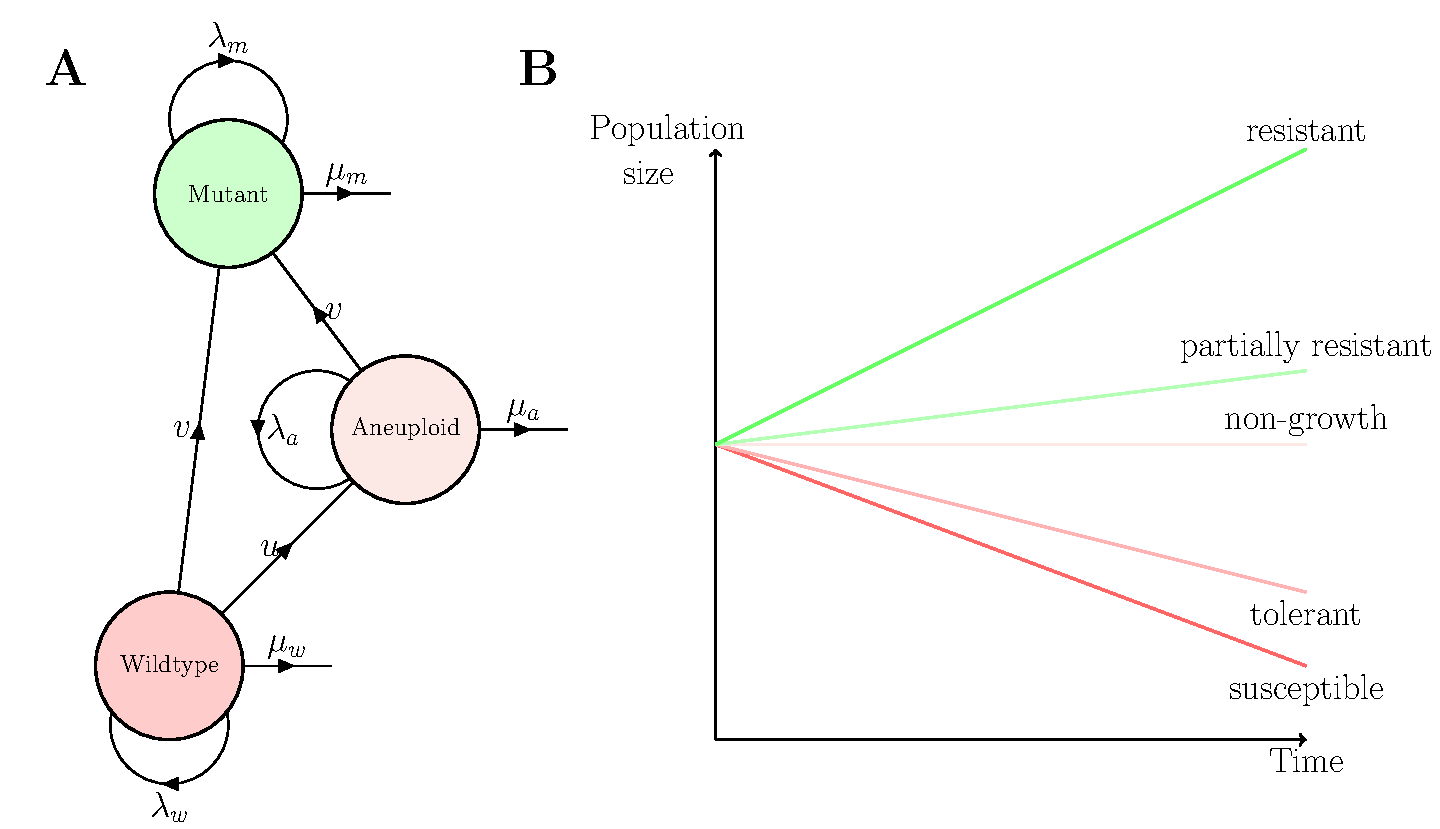
\includegraphics[width=\textwidth]{Figures/figureAneuploidy.pdf}
\caption{
\textbf{Model illustration.}
\textbf{(A)} A population of cancer cells is composed of wildtype, aneuploid, and mutant cells, which divide with rates $\lambda_w$, $\lambda_a$, and $\lambda_m$ and die at rates $\mu_w$, $\mu_a$, and $\mu_m$, respectively. 
Wildtype cells can become aneuploid at rate $u$. Both aneuploid and wildtype cells can acquire a beneficial mutation with rate $v$. Color denotes the relative growth rates of the three genotypes such that $\lambda_w - \mu_w < \lambda_a - \mu_a < \lambda_m - \mu_m$. \textbf{(B)} The wildtype and the mutant are susceptible and resistant, respectively, to the drug. The aneuploid may be tolerant $(4)$, non-growing $(3)$, partially resistant $(2)$ or fully resistant $(1)$.
}
\label{figureAneuploidy}
\end{figure}

%%%%%%%%%%%
% Fig 3A: prob rescue vs N for various Delta_a; markup N*
% Fig 3B: N* vs Delta_a
% Fig 3C: N* vs u/v

\begin{figure}
\begin{subfigure}{0.5\textwidth}
A\\
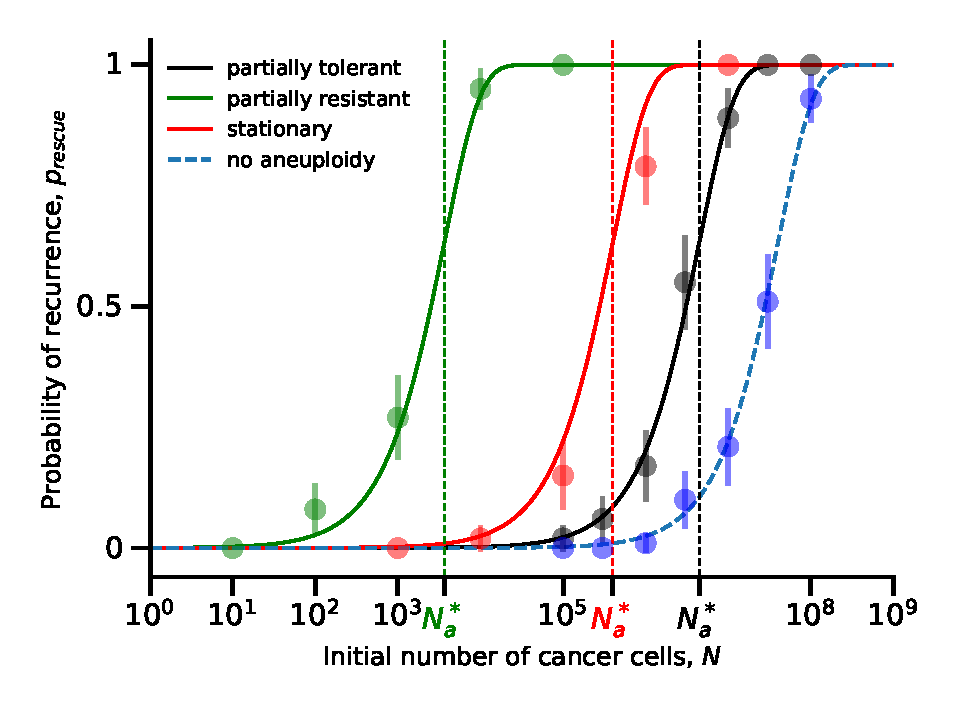
\includegraphics[width=1\textwidth]{Figures/ProbvNPlot.pdf}
\end{subfigure}
\\
\begin{subfigure}{0.5\textwidth}
B\\
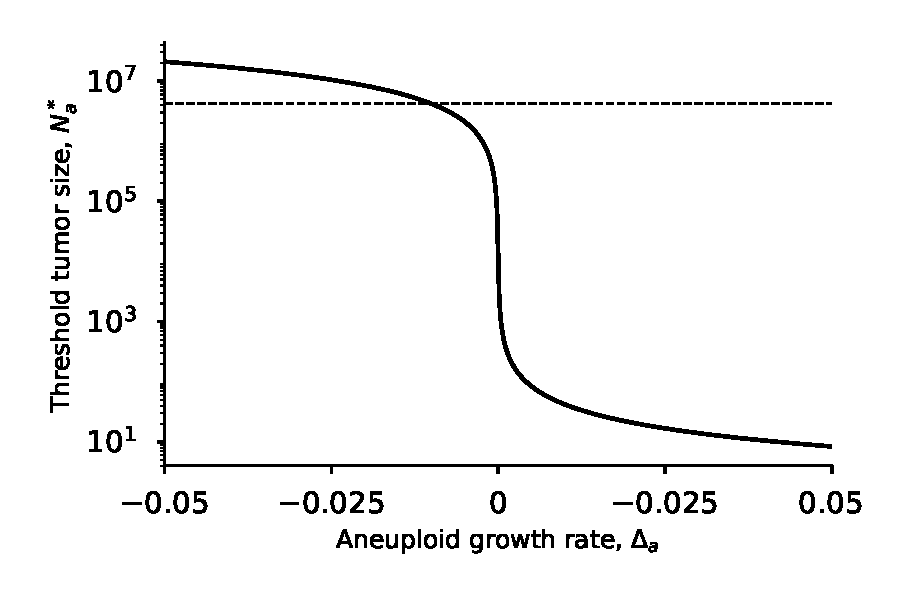
\includegraphics[width=1\textwidth]{Figures/ThresholdPopulationSizePlot.pdf}
\end{subfigure}
\begin{subfigure}{0.5\textwidth}
C\\
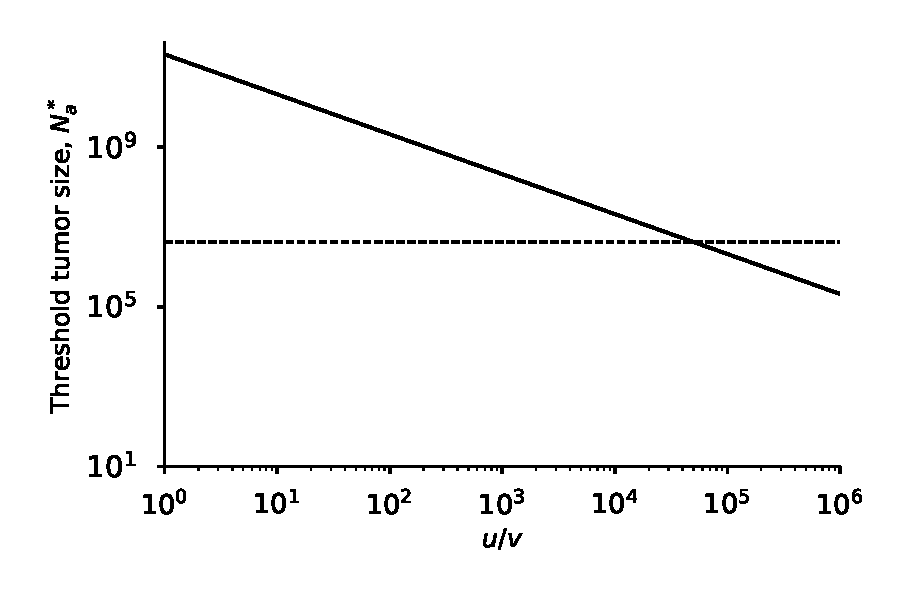
\includegraphics[width=1\textwidth]{Figures/ThresholdPopulationSizeVersusRatioPlot.pdf}
\end{subfigure}
\caption{
\textbf{Aneuploidy facilitates evolutionary rescue of cancer under drug treatment.}
\textbf{(A)} The probability of evolutionary rescue (i.e. the probability that the population does not go to extinction), $\presc$, as a function of the initial tumor size, $N$. Dashed vertical line shows the threshold tumor size, $N_a^*$, above which the probability is very high. Blue dashed line represents the probability of evolutionary rescue as a function of $N$ without aneuploidy ($u=0$). The blue and and red dots represent numerical simulations for the case with aneuploidy and without aneuploidy, respectively. The error bars represent $95\%$ confidence interval of the form $p\pm1.96\sqrt{p\left(1-p\right)/n}$ where $p$ is the  probability of that a succesful mutant has not ben generated and $n=100$ is the number of simulations.
\textbf{(B)} The threshold tumor size $N_a^*$ as a function of the aneuploid growth rate $\Delta_a$. The dashed horizontal line shows $N^*_m$, the threshold tumor size without aneuploidy ($u=0$). The red dots represent numerical simulations.  The inset highlights the case when aneuploidy cancer cells are non-growing. When aneuploid growth rate is close to or higher than zero, aneuploidy decreases the threshold tumor size, thereby facilitating evolutionary rescue. 
\textbf{(C)} The threshold tumor size $N_a^*$ as a function of the ratio of aneuploidy and mutation rates, $u/v$. The dashed horizontal line shows $N^*_m$, the threshold tumor size without aneuploidy ($u=0$). The blue line represents the exact formula for threshold tumor size $N_a^*$. The red dots represent numerical simulations.  When the aneuploidy rate is much higher than the mutation rate, aneuploidy decreases the threshold tumor size, thereby facilitating evolutionary rescue.
}
\label{rescue_prob}
\end{figure}
%%%%%%%%%%%
\begin{figure}
\vspace*{1\baselineskip}
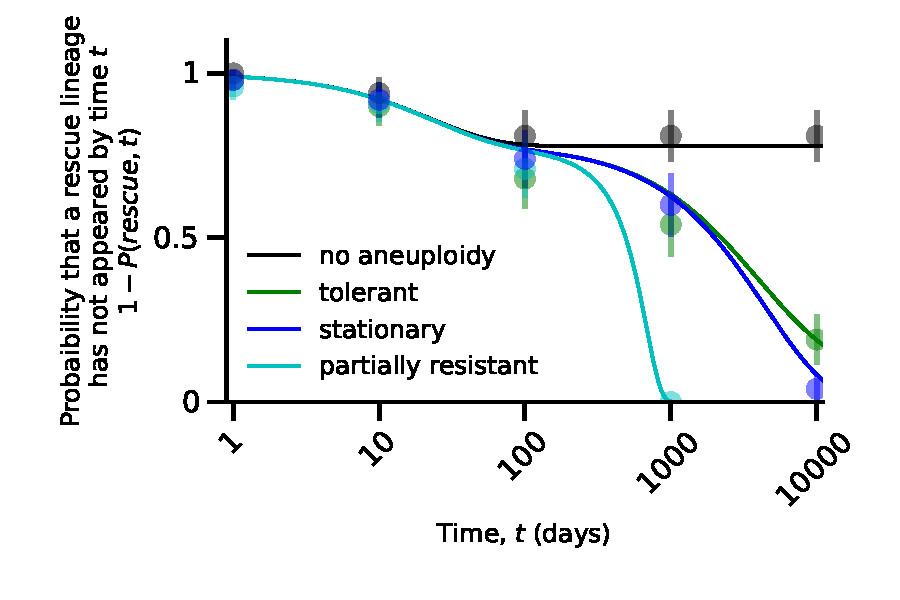
\includegraphics[width=1\textwidth]{Figures/ReboundProbability.pdf}
\caption{Plot of the probability that a succesful mutant has not appeared by time $t$. The blue line represents the case with aneuploidy ($u>0$), the black line represents the case without aneuploidy ($u=0$).  The green and and red dots represent numerical simulations for the case with aneuploidy and without aneuploidy, respectively.  For the simulations we have chosen the following parameters: $\lambda_w=0.14, \lambda_a=0.14,\lambda_m=0.14,\mu_w=0.17,\mu_a=0.1401,\mu_m=0.13, u=0.14\times10^{-2}, v=0.14\times10^{-7}$. The error bars represent $95\%$ confidence interval of the form $p\pm1.96\sqrt{p\left(1-p\right)/n}$ where $p$ is the  probability of that a succesful mutant has not ben generated and $n=100$ is the number of simulations. As time increases, aneuploidy plays an important role in helping the cancer cell population escape extinction.}
\label{ReboundProbability}
\end{figure}
%%%%%%%%%%%

%%%%%%%%%%%%
%
%\begin{figure}
%\begin{subfigure}{0.5\textwidth}
%\includegraphics[width=1\textwidth]{Figures/FILENAME.pdf}
%\end{subfigure}
%\begin{subfigure}{0.5\textwidth}
%\includegraphics[width=1\textwidth]{Figures/FILENAME.pdf}
%\end{subfigure}
%\caption{
%\textbf{TITLE}
%CAPTION
%}
%\label{fig:LABEL}
%\end{figure}
%%%%%%%%%%%%

%%%%%%%%%%%%
%
%\begin{figure}
%\begin{subfigure}{0.5\textwidth}
%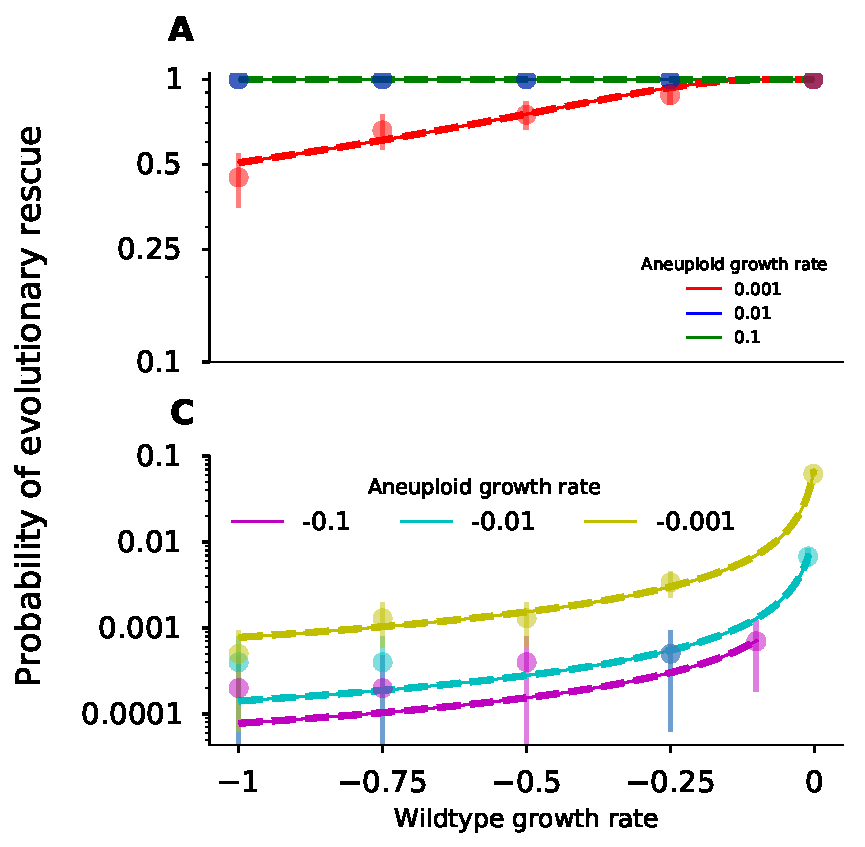
\includegraphics[width=1\textwidth]{Figures/CombinedSubplot.pdf}
%\end{subfigure}
%\begin{subfigure}{0.5\textwidth}
%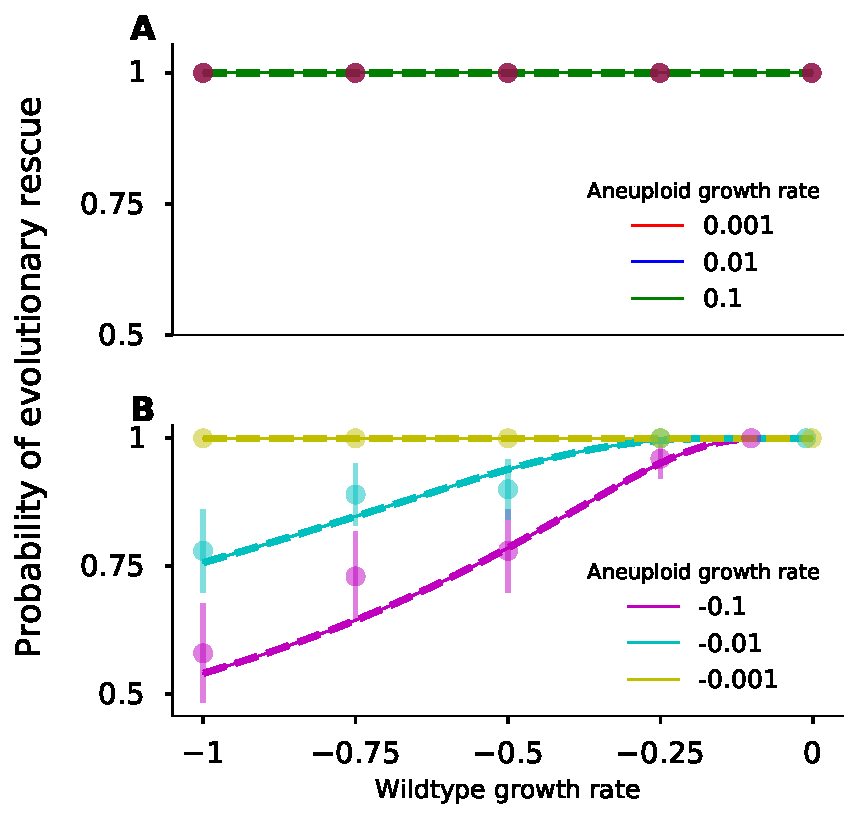
\includegraphics[width=1\textwidth]{Figures/CombinedSubplotLargePop.pdf}
%\end{subfigure}
%\caption{
%\textbf{Evolutionary rescue probability with partially resistant or tolerant aneuploid cells.}
%Rescue probability is very high when aneuploidy provides partial resistance ($\lambda_a=0.01$), in an initially small tumor (\textbf{A}, $N=10^4$) and even more so in an initially large tumor (\textbf{B}, $N=10^8$). 
%When aneuploidy provides tolerance (\textbf{C}, $N=10^4$; \textbf{D}, $N=10^8$), the rescue probability is much lower. 
%In both scenarios, rescue probability increase with both the wildtype growth rate (x-axis) and the aneuploidy growth rate (colors).
%Markers represent simulation results with 95\% CI; solid and dashed lines for the exact formula (\cref{eq:survival_prob} in \cref{eq:rescue_prob}); dashed lines for the approximate formula (\cref{rescue_prob_approx}), demonstrating that they all agree.
%Parameters: division rate $\lambda_w=\lambda_a=\lambda_m=0.14$ (so that growth rate changes due to variable death rate); mutant death rate $\mu_m=0.13$ (so that mutant growth rate $\Delta_m=0.01$); aneuploidy rate $u=10^{-2}$; mutation rate $v=10^{-7}$.
%}
%\label{rescue_prob_wt_growth}
%\end{figure}
%%%%%%%%%%%%

%\begin{figure}
%% small population size
%% switch from tolerance to non-growing
%% TODO why no switch in panel B?
%% TODO more simulations for 0 > Delta_a > Delta^*_a
%% TODO simulations in A?
%\begin{subfigure}{0.5\textwidth}
%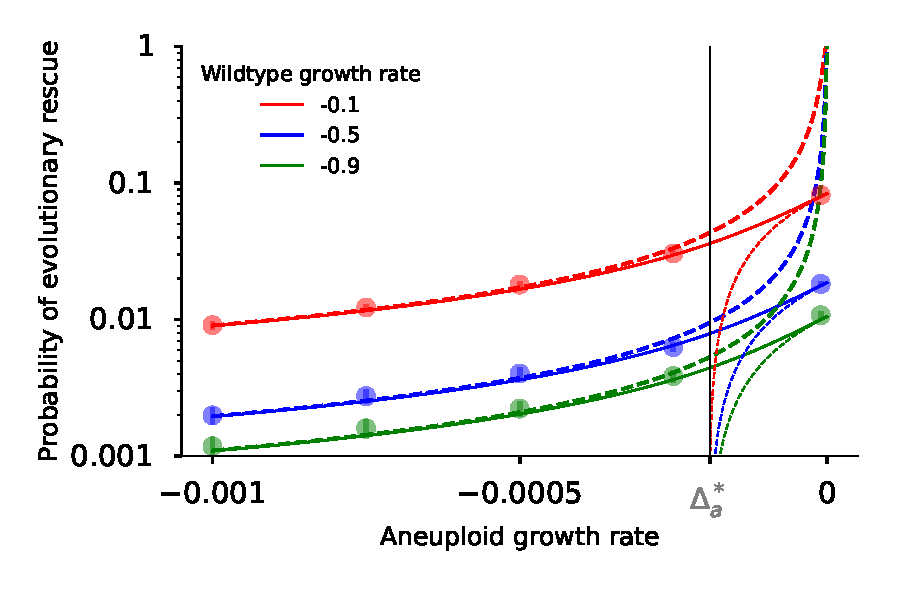
\includegraphics[width=1\textwidth]{Figures/P_est_divergence.pdf}
%\end{subfigure}
%\begin{subfigure}{0.5\textwidth}
%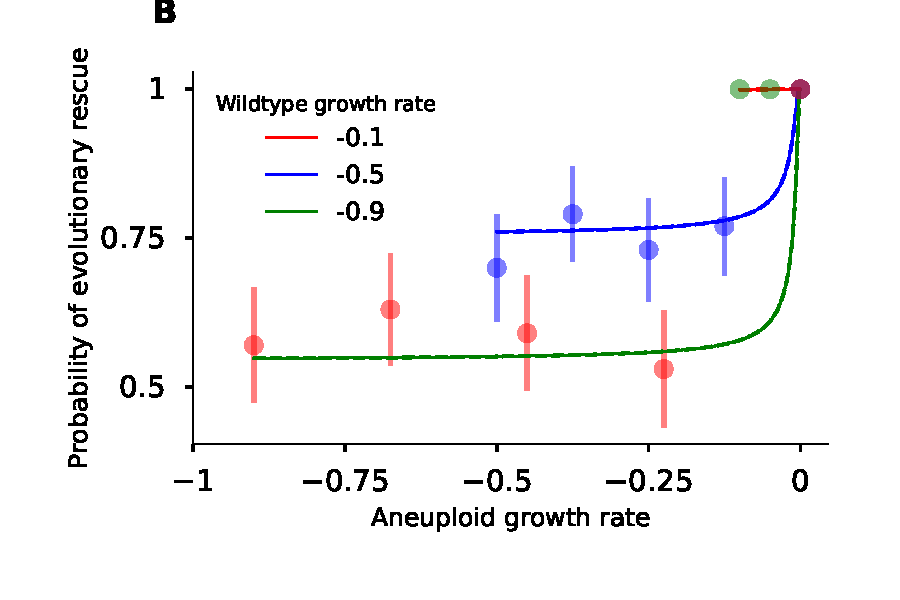
\includegraphics[width=1\textwidth]{Figures/P_est_divergenceLargePopulation.pdf}
%\end{subfigure}
%\caption{\textbf{Evolutionary rescue probability with tolerant or non-growing aneuploid cells.}
%Rescue probability grows with the aneuploid growth rate $\Delta_a$ (x-axis), and is much higher in an initially large tumor than in a small one (\textbf{A}: $N=10^4$; \textbf{B}: $N=10^8$). 
%Markers for simulation results with 95\% CI; 
%solid lines for the exact formula (\cref{eq:survival_prob} in \cref{eq:rescue_prob});
%dashed lines for the approximate formula (\cref{rescue_prob_approx}).
%The approximation agrees with the simulation and exact solution when the initial tumor size is large (panel B).
%When the tumor size is small (panel A), we switch between the approximation for tolerant and for non-growing aneuploid cells; the switch occurs at $1/T^*$. % TODO ref to eq
%Parameters: $\lambda_w=\lambda_a=\lambda_m=0.14$; $\mu_m=0.13$; $u=10^{-2}$; $v=10^{-7}$.
%}
%\label{rescue_prob_an_growth}
%\end{figure}

%%%%%%%%%%%%


%%%%%%%%%%%%
%
%\begin{figure}
%% slightly decreasing (need to check)
% \vspace*{1\baselineskip}
%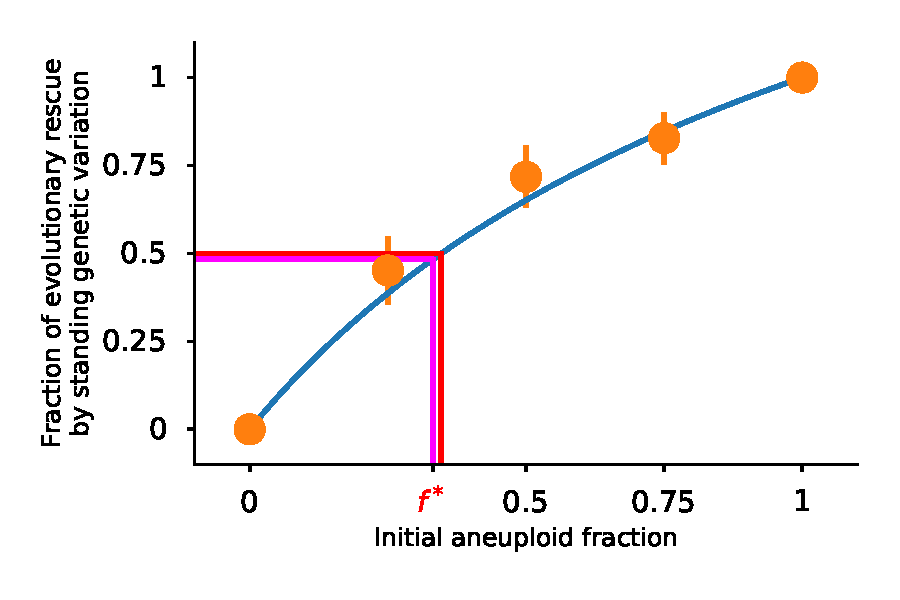
\includegraphics[width=1\textwidth]{Figures/FractionPlot.pdf}
%\caption{\textbf{Effect of standing variation on evolutionary rescue.}
%In aneuploid cells already exist in the population at the onset of drug therapy as standing genetic variation, then evolutionary rescue is more likely... 
%Parameters: $\lambda_w=\lambda_a=\lambda_m=0.14$; $\mu_w=0.17$; $\mu_a=0.145$; $\mu_m=0.13$; $u=10^{-2}$; $v=10^{-7}$.
%% TODO think about this figure...
%% TODO maybe better to show p_total / p_denovo as function of u or N.
%}
%\label{FractionPlot}
%\end{figure}
%
%%%%%%%%%%%%
%
%\begin{figure}
%\begin{subfigure}{0.5\textwidth}
%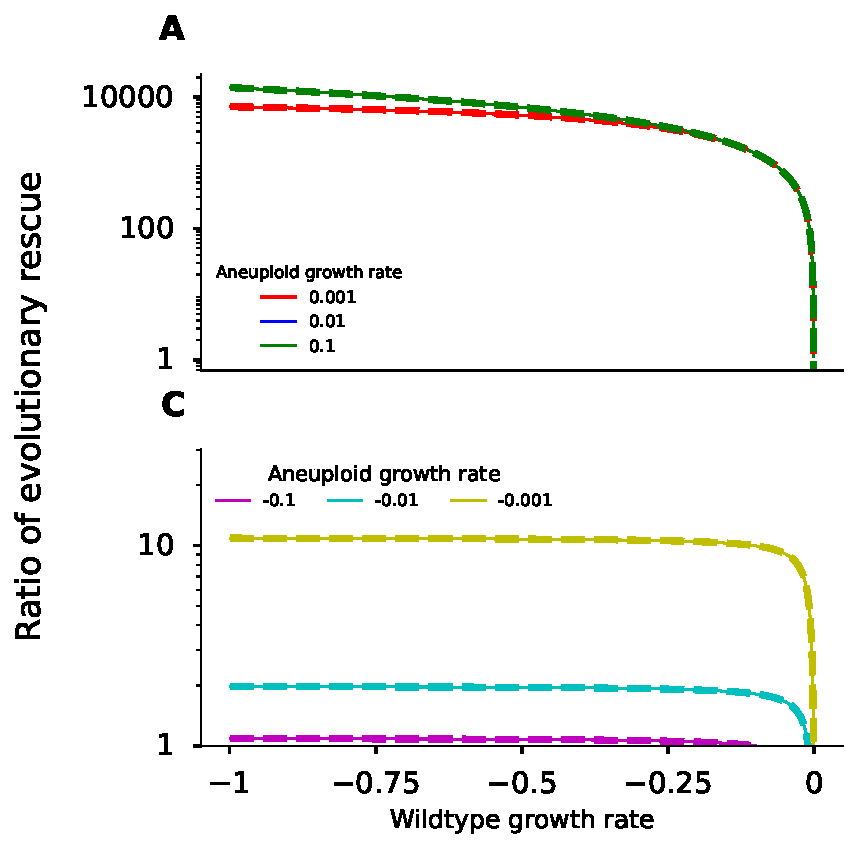
\includegraphics[width=1\textwidth]{Figures/RatioEvolRescue.pdf}
%\end{subfigure}
%\begin{subfigure}{0.5\textwidth}
%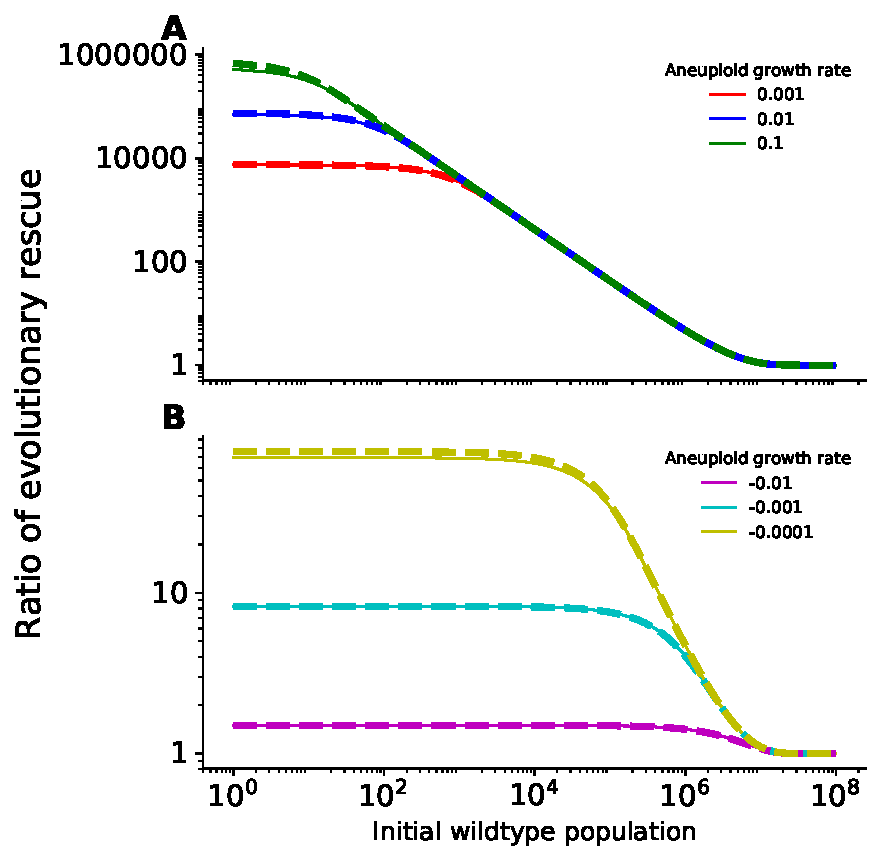
\includegraphics[width=1\textwidth]{Figures/RatioEvolRescuePopulationSize.pdf}
%\end{subfigure}
%\caption{\textbf{Effect of aneuploidy on evolutionary rescue.}
%The ratio of rescue probability with and without aneuploid ($H$, \cref{ratiorescue}) increases with the aneuploid growth rate (colors) and decreases with the wildtype growth rates and initial tumor size (x-axes), except for large tumors where where the ratio converges to unity.
%\textbf{(A, B)} Aneuploidy provides partial resistance.
%\textbf{(C, D)} Aneuploidy provides tolerance.  
%Solid and dashed lines apply $p_{rescue}$ from the exact formula of  (\cref{eq:survival_prob} in \cref{eq:rescue_prob}); dashed lines apply $p_{rescue}$ from the approximate formula (\cref{rescue_prob_approx}), with good agreement.
%Parameters: $N=10^4$; $\lambda_w=\lambda_a=\lambda_m=0.14$; (B) $\mu_w=0.17$; $\mu_m=0.13$; $u=10^{-2}$; $v=10^{-7}$.
%% TODO start y at 1
%}
%\label{rescue_ratio}
%\end{figure}
%
%%%%%%%%%%%%

%%%%%%%%%%%%
%
%\begin{figure}
% \vspace*{1\baselineskip}
%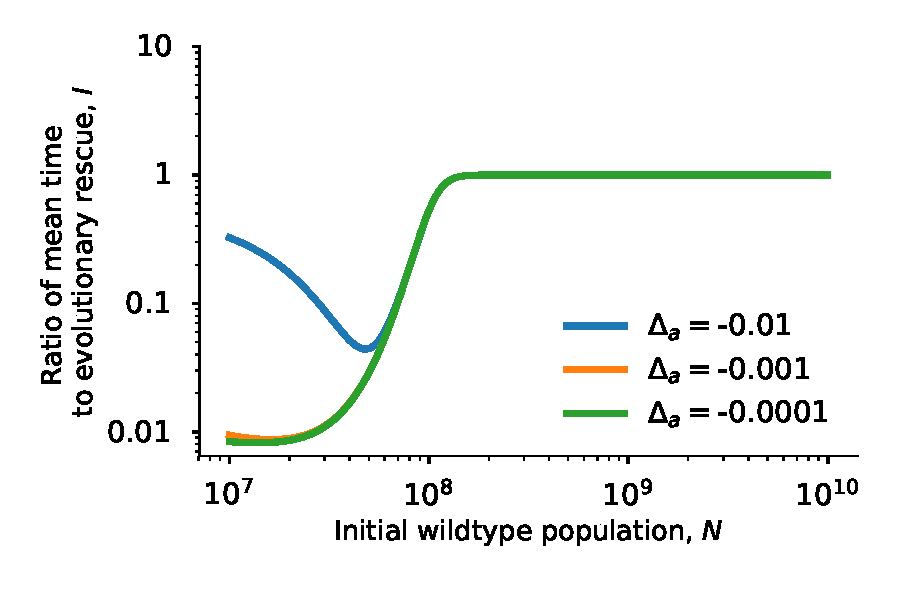
\includegraphics[width=1\textwidth]{Figures/MeanTimeRatioInitialPopulationSize.pdf}
%\caption{\textbf{Ratio of evolutionary rescue time with and without aneuploidy.}
%The ratio of the mean time to appearance of a resistance mutation that leads to evolutionary rescue with ($u>0$) and without ($u=0$) aneuploidy for variable initial tumor sizes (\cref{eq:eqMeanTimeRatioInitialPopulationSize}) when aneuploidy provides tolerance to the drug ($\Delta_a < 0$). When the initial tumor size is not large ($<10^8$), aneuploidy can decrease the rescue time by 10-100-fold.
%% TODO parameter values 
%}
%\label{MeanTimeRatioInitialPopulationSize}
%\end{figure}
%
%%%%%%%%%%%%

%%%%%%%%%%
%
%\begin{figure}
%% diffusion approx instead of branching process
%% tolerance
% \vspace*{1\baselineskip}
%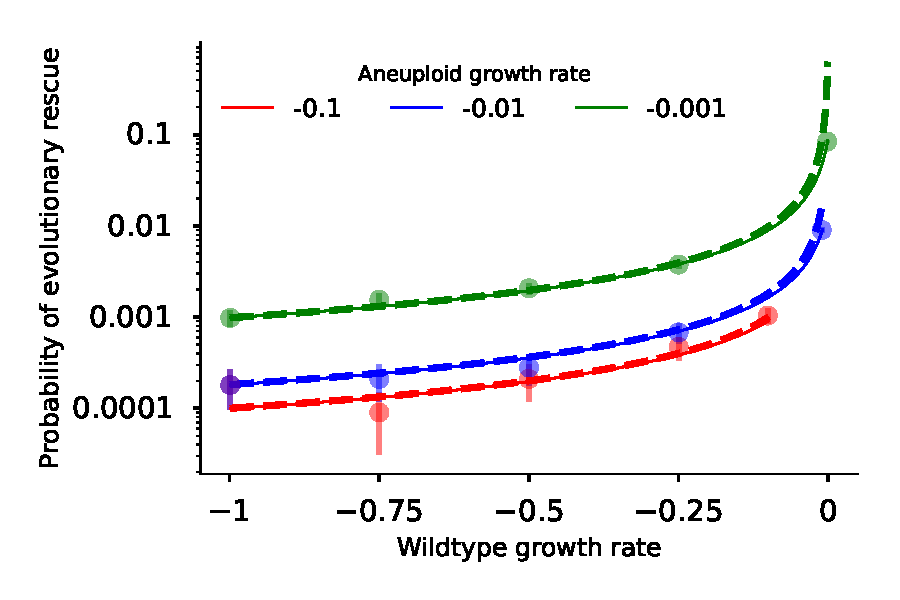
\includegraphics[width=1\textwidth]{Figures/P_est_diffusion.pdf}
%\caption{Plot of the survival probability of an initial population consisting of $w_0=10^{4}$ wildtype cells as a function of $\Delta_a=\lambda_a-\mu_a$ for various values of $\Delta_w=\lambda_a-\mu_a$. The continuous lines represent the exact result \eqref{survprobw} while the dashed lines represent the Feller diffusion approximation \eqref{FellerApprox}. The error bars represent $95\%$ confidence interval of the form $p\pm1.96\sqrt{p\left(1-p\right)/w_0}$ where $p$ is the mean probability of evolutionary rescue.}
%\label{P_est_diffusion}
%\end{figure}
%
%%%%%%%%%%%
%
%\begin{figure}
%% partial resistance, compare 1st and 2nd order approximation and exact
%\vspace*{1\baselineskip}
%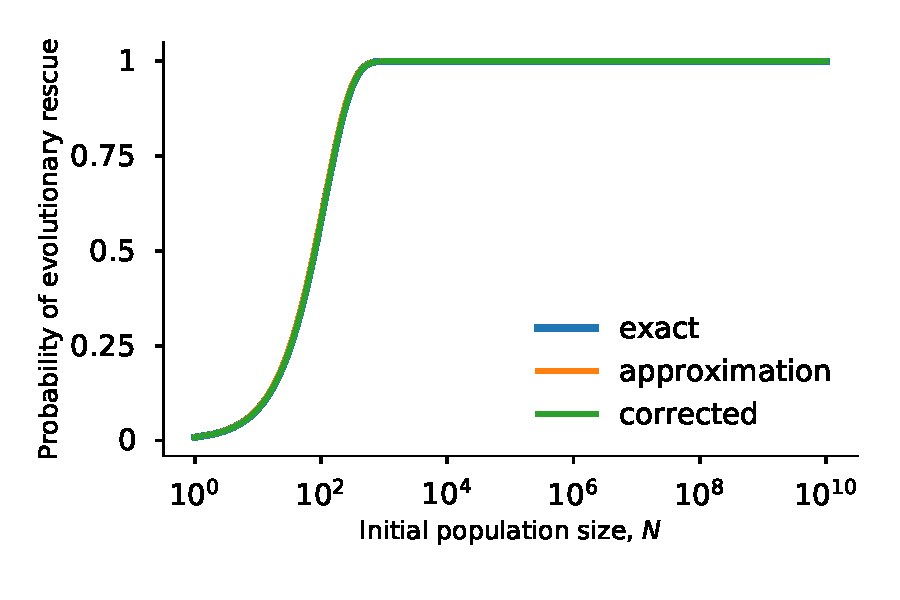
\includegraphics[width=1\textwidth]{Figures/SurvPlotNData.pdf}
%\caption{Plot of the probability of survival of a population as a function of the initial population size of wildtype cells. The blue line represents the exact solution \eqref{survprobw}, the orange line line represents the approximation \eqref{aneuploidyresistentfirstapprox}, the green line represents the first order correction \eqref{survprobwapproxcorrected} and the red dots represents stochastic simulations. For the simulations we have chosen the following parameters: $\lambda_w=0.14, \lambda_a=0.14,\lambda_m=0.14,\mu_w=0.17,\mu_a=0.135,\mu_m=0.13$. The error bars represent $95\%$ confidence interval of the form $p\pm1.96\sqrt{p\left(1-p\right)/n}$ where $p$ is the mean probability of evolutionary rescue and $n=100$ is the number of simulations.}
%\label{compare_1st_2nd_order_approx}
%\end{figure}

%%%%%%%%%%%%%%%%%%%%%%%%%%%%%%%%%%%%%%%%%%

\newpage 
\clearpage

\begin{appendices}
\renewcommand{\theequation}{\thesection\arabic{equation}}
\counterwithin*{equation}{section}

%%%%%%%%%%%%%%%%%%%%%%%%%%%%%%%%%%%%%
\section*{Appendix A: Survival probability of a single lineage}\label{sec:appendix-surv-prob}

To analyze evolutionary rescue in this model, we use the framework of \emph{multitype branching processes} \citep{harris1963theory, weissman2009rate}. 
This allows us to find explicit expressions for the \emph{survival probability}: the probability that a lineage descended from a single cell does not become extinct.

Let $p_w$, $p_a$, and $p_m$ be the survival probabilities of a population consisting initially of single wildtype cell, aneuploid cell, or mutant cell, respectively.
The complements $1-p_w$, $1-p_a$, and $1-p_m$ are the extinction probabilities, which satisfy each its respective equation,
\begin{equation} \label{eq:extinction_prob}
\begin{aligned}
1-p_w = &\frac{\mu_w}{\lambda_w+\mu_w+u+v} + 
		  \frac{u}{\lambda_w+\mu_w+u+v}\left(1-p_a\right) + \\
		  & \frac{\lambda_w}{\lambda_w+\mu_w+u+v}\left(1-p_w\right)^2 +
		  \frac{v}{\lambda_w+\mu_w+u+v}\left(1-p_m\right) ,\\
1-p_a = &\frac{\mu_a}{\lambda_a+\mu_a+v}+\frac{v}{\lambda_a+\mu_a+v}\left(1-p_m\right)+\frac{\lambda_a}{\lambda_a+\mu_a+v}\left(1-p_a\right)^2 ,\\
1-p_m = &\frac{\mu_m}{\lambda_m+\mu_m}+\frac{\lambda_m}{\lambda_m+\mu_m}\left(1-p_m\right)^2 .	 
\end{aligned}
\end{equation}

The survival probabilities are given by the smallest solution for each quadratic equation \citep{uecker2015adaptive}. Therefore we have
\begin{equation}\label{eq:survival_prob}
\begin{aligned}
p_w &= \frac{\lambda_w-\mu_w-u-v+\sqrt{\left(\lambda_w-\mu_w-u-v\right)^2+4\lambda_w\left(up_a+vp_m\right)}}{2\lambda_w} ,\\
p_a &= \frac{\lambda_a-\mu_a-v+\sqrt{\left(\lambda_a-\mu_a-v\right)^2+4\lambda_avp_m}}{2\lambda_a}, \\
p_m &= \frac{\lambda_m-\mu_m}{\lambda_m} .
\end{aligned} 
\end{equation}
Note that the equation for $p_w$ depends on both $p_a$ and $p_m$, and the equation for $p_a$ depends on $p_m$.
To proceed, we can plug the solution for $p_m$ and $p_a$ into the solution for $p_w$. We perform this for three different scenarios.

%%%%%%%%%%%%%%%%%%%%%%%%%%%%%%%%%%%%%
\subsubsection*{Scenario 1: Aneuploid cells are partially resistant} 

We first assume that aneuploidy provides partial resistance to drug therapy, $\lambda_a>\mu_a$, and that this resistance is significant, $\left(\lambda_a-\mu_a-v\right)^2 > 4\lambda_a v p_m$.
We thus rewrite \cref{eq:survival_prob} as
\begin{align*}
p_w&=\frac{\lambda_w-\mu_w-u-v}{2\lambda_w}\left(1-\sqrt{1+\frac{4\lambda_w\left(vp_m+up_a\right)}{\left(\lambda_w-\mu_w-u-v\right)^2}}\right) ,
\text{and} \\
p_a&=\frac{\lambda_a-\mu_a-v}{2\lambda_a}\left(1+\sqrt{1+\frac{4\lambda_avp_m}{\left(\lambda_a-\mu_a-v\right)^2}}\right) . 
\end{align*}
Using the quadratic Taylor expansion $\sqrt{1+x}=1+x/2+\mathcal{O}(x^2)$ and assuming $u,v \ll 1$,
we obtain the following approximation for the survival probability of a population initially consisting of a single wildtype cell,
\begin{align} \label{eq:survprobwapprox1}
p_w 
&\approx -\frac{vp_m+up_a}{\lambda_w-\mu_w-u-v}\\
\nonumber
%&\approx-\frac{1}{\lambda_w-\mu_w-u-v}\left[\frac{v\left(\lambda_a-\mu_a-u\right)}{\lambda_a}+\frac{uv\left(\lambda_m-\mu_m\right)}{\lambda_m\left(\lambda_a-\mu_a-u\right)}+\frac{v\left(\lambda_m-\mu_m\right)}{\lambda_m}\right]\\ \label{survprobw2}
&\approx-\frac{1}{\lambda_w-\mu_w}\left[\frac{u\left(\lambda_a-\mu_a\right)}{\lambda_a}+\frac{uv\left(\lambda_m-\mu_m\right)}{\lambda_m\left(\lambda_a-\mu_a\right)}+\frac{v\left(\lambda_m-\mu_m\right)}{\lambda_m}\right]\\
\end{align}
Now $u v$ is very small, and if we assume $v \ll u$, we have
\begin{equation}
p_w \approx \frac{u}{\abs{\Delta_w}} \cdot \frac{\Delta_a}{\lambda_a} .
\end{equation}

%%%%%%%%%%%%%%%%%%%%%%%%%%%%%%%%%%%%%
\paragraph{Second-order approximation.} 
To improve our approximation, we can consider the second term of the Taylor series expansion,
\begin{align*}
\left(1+\frac{4\lambda_avp_m}{\left(\lambda_a-\mu_a-v\right)^2}\right)^{\frac{1}{2}}=1+\frac{2\lambda_avp_m}{\left(\lambda_a-\mu_a-v\right)^2}-\frac{\left(\lambda_avp_m\right)^2}{4\left(\lambda_a-\mu_a-v\right)^4}+\cdots,
\end{align*}
which gives us the following approximation,
\begin{align}
p_a \approx \frac{\lambda_a-\mu_a-v}{\lambda_a}+\frac{vp_m}{\lambda_a-\mu_a-v}-\frac{\lambda_a\left(vp_m\right)^2}{8\left(\lambda_a-\mu_a-v\right)^3} .
\end{align}
We therefore have
\begin{align}\nonumber
p_w&\approx-\frac{1}{\lambda_w-\mu_w-u-v}\left[\frac{u\left(\lambda_a-\mu_a-v\right)}{\lambda_a}+\frac{uv\left(\lambda_m-\mu_m\right)}{\lambda_m\left(\lambda_a-\mu_a-v\right)}+\frac{v\left(\lambda_m-\mu_m\right)}{\lambda_m}-\frac{uv^2\lambda_a\left(\lambda_m-\mu_m\right)^2}{8\lambda_m^2\left(\lambda_a-\mu_a-v\right)^3}\right]\\ \label{survprobw3}
&\approx-\frac{1}{\lambda_w-\mu_w}\left[\frac{u\left(\lambda_a-\mu_a\right)}{\lambda_a}+\frac{uv\left(\lambda_m-\mu_m\right)}{\lambda_m\left(\lambda_a-\mu_a\right)}+\frac{v\left(\lambda_m-\mu_m\right)}{\lambda_m}-\frac{uv^2\lambda_a\left(\lambda_m-\mu_m\right)^2}{8\lambda_m^2\left(\lambda_a-\mu_a\right)^3}\right], 
\end{align}
and using $\Delta_k=\lambda_k-\mu_k$, we can write the above equation as
\begin{equation}\label{survprobwapproxcorrected}
p_w \approx -\frac{1}{\Delta_w}\left(\frac{u\Delta_a}{\lambda_a}+\frac{uv\Delta_m}{\lambda_m\Delta_a}+\frac{v\Delta_m}{\lambda_m}-\frac{uv^2\lambda_a\Delta_m^2}{8\lambda_m^2\Delta_a^3}\right).
\end{equation}


%%%%%%%%%%%%%%%%%%%%%%%%%%%%%%%%%%%%%
\subsubsection*{Scenario 2: Aneuploid cells are tolerant.} 

We now assume that aneuploidy provides tolerance to drug therapy, that is, the number of aneuploid cells significantly declines over time, but at a lower rate than the number of wildtype cells, $\lambda_w - \mu_w < \lambda_a - \mu_a < 0$. We also assume that the decline are significant, $\left(\lambda_a-\mu_a-v\right)^2 > 4\lambda_a v p_m$.
We rewrite \cref{eq:survival_prob} as
\begin{equation}
\begin{aligned}
p_w&=\frac{\lambda_w-\mu_w-u-v}{2\lambda_w}\left(1-\sqrt{1+\frac{4\lambda_w\left(vp_m+up_a\right)}{\left(\lambda_w-\mu_w-u-v\right)^2}}\right) ,
\text{and} \\
p_a&=\frac{\lambda_a-\mu_a-v}{2\lambda_a}\left(1-\sqrt{1+\frac{4\lambda_avp_m}{\left(\lambda_a-\mu_a-v\right)^2}}\right) .
\end{aligned}
\end{equation}
Since $u,v\ll1$, the term in the root can be approximated using a 1st-order Taylor expansion. So, substituting the expressions for $p_a$ and $p_m$, we have
\begin{equation} \label{eq:survprobwinitial}
\begin{aligned}
p_w&\approx-\frac{vp_m+up_a}{\lambda_w-\mu_w-u-v}\\
&\approx\frac{1}{\lambda_w-\mu_w-u-v}\left[\frac{uv\left(\lambda_m-\mu_m\right)}{\lambda_m\left(\lambda_a-\mu_a-v\right)}-\frac{v\left(\lambda_m-\mu_m\right)}{\lambda_m}\right]\\ %\label{survprobw2}
&\approx\frac{v\left(\lambda_m-\mu_m\right)}{\lambda_m\left(\lambda_w-\mu_w\right)}\left[\frac{u}{\left(\lambda_a-\mu_a\right)}-1\right] \\
&=\frac{v\Delta_m}{\lambda_m \abs{\Delta_w}}\left(\frac{u}{\abs{\Delta_a}}+1\right) .
\end{aligned}
\end{equation}
If we assume that $u>\abs{\Delta_a}$ then we have:
\begin{equation*}
p_w\approx\frac{u}{\abs{\Delta_w}}\cdot\frac{v\Delta_m}{\lambda_m \abs{\Delta_a}}.
\end{equation*}

%%%%%%%%%%%%%%%%%%%%%%%%%%%%%%%%%%%%%
\subsubsection*{Scenario 3: Aneuploid cells are non-growing} % TODO consider this name ok

We now assume that the growth rate of aneuploid cells is close to zero (either positive or negative), such that  $\left(\lambda_a-\mu_a-v\right)^2 < 4\lambda_avp_m$.
We rewrite \cref{eq:survival_prob} as
\begin{equation}
p_a = \frac{\lambda_a-\mu_a-v+2\sqrt{\lambda_a vp_m}\left(1+\frac{\left(\lambda_a-\mu_a-v\right)^2}{4\lambda_avp_m}\right)^{\frac12}}{2\lambda_a} .
\end{equation}
Using a following Taylor series expansion for small $\left(\lambda_a-\mu_a-v\right)^2 / 4\lambda_avp_m$,
\begin{equation*}
\left(1+\frac{\left(\lambda_a-\mu_a-v\right)^2}{4\lambda_avp_m}\right)^{\frac{1}{2}}=1+\frac{\left(\lambda_a-\mu_a-v\right)^2}{8\lambda_avp_m}+\cdots,
\end{equation*}
we obtain the approximation
\begin{equation}
\begin{aligned}
p_a&\approx\frac{\lambda_a-\mu_a-v+2\sqrt{\lambda_a vp_m}\left[1+\frac{\left(\lambda_a-\mu_a-v\right)^2}{8\lambda_avp_m}\right]}{2\lambda_a}\\
&=\frac{\lambda_a-\mu_a-v+2\sqrt{\lambda_a vp_m}+\frac{\left(\lambda_a-\mu_a-v\right)^2}{4\sqrt{\lambda_avp_m}}}{2\lambda_a}\\
&=\frac{\left(\lambda_a-\mu_a-v+2\sqrt{\lambda_avp_m}\right)^2+4\lambda_avp_m}{8\lambda_a\sqrt{\lambda_avp_m}}\\
&=\frac{4\lambda_avp_m+4\lambda_avp_m\left(1+\frac{\lambda_a-\mu_a-v}{2\sqrt{\lambda_avp_m}}\right)^2}{8\lambda_a\sqrt{\lambda_avp_m}}\\
&=\frac{1}{2\lambda_a}\left(\lambda_a-\mu_a-v+2\sqrt{\lambda_avp_m}\right).
\end{aligned}
\end{equation}
Plugging this in \cref{eq:survprobwinitial}, the survival probability of a population starting from one wildtype individual is
\begin{equation}\label{eq:scenario3}
\begin{aligned}
p_w&\approx-\frac{1}{\lambda_w-\mu_w-u-v}\left[v\frac{\lambda_m-\mu_m}{\lambda_m}+\frac{u}{2\lambda_a}\left(\lambda_a-\mu_a-v+2\sqrt{\lambda_avp_m}\right)\right]\\
&=-\frac{1}{\lambda_w-\mu_w-u-v}\left[v\frac{\lambda_m-\mu_m}{\lambda_m}+\frac{u}{2\lambda_a}\left(\lambda_a-\mu_a-v\right)+u\sqrt{\frac{v\left(\lambda_m-\mu_m\right)}{\lambda_a\lambda_m}}\right]\\
&\approx-\frac{1}{\Delta_w}\left[v\frac{\Delta_m}{\lambda_m}+\frac{u\left(\Delta_a-v\right)}{2\lambda_a}+u\sqrt{\frac{v\Delta_m}{\lambda_a\lambda_m}}\right].
\end{aligned}
\end{equation}
Using the fact that
\begin{equation*}
\left(\Delta_a-v\right)^2 < 4\lambda_avp_m\Rightarrow\frac{\Delta_a-v}{2\lambda_a} < \sqrt{\frac{v\Delta_m}{\lambda_a\lambda_m}},
\end{equation*}
and $v\ll u$ we obtain:
\begin{equation}
p_w\approx\frac{u}{\abs{\Delta_w}}\cdot\sqrt{\frac{v\Delta_m}{\lambda_a\lambda_m}}.
\end{equation}
%%%%%%%%%%%%%%%%%%%%%%%%%%%%%%%%%%%%%%%%%%

\section*{Appendix B: Evolutionary rescue probability}\label{sec:appendix-rescue-prob}

Substituting \cref{eq:survprobwapprox1,eq:survprobwinitial,eq:scenario3} into \cref{eq:rescue_prob}, the evolutionary rescue probability can be approximated by
\begin{equation}\label{rescue_prob_approx}
\begin{aligned}
&\presc \approx \\
  &\begin{cases}
  1-\exp\left[\frac{N}{\Delta_w-u-v}\left(v\frac{\Delta_m}{\lambda_m}+\frac{u\left(\Delta_a-v\right)}{2\lambda_a}+u\sqrt{\frac{v\Delta_m}{\lambda_a\lambda_m}}\right)\right] ,&
  4\lambda_avp_m>\left(\Delta_a-v\right)^2 ,\\
   1-\exp\left[\frac{v\Delta_mN}{\lambda_m\Delta_w}\left(1-\frac{u}{\Delta_a}\right)\right] ,&
   \Delta_a<0\quad\text{and}\quad4\lambda_avp_m<\left(\Delta_a-v\right)^2 ,\\
   1-\exp\left[\frac{N}{\Delta_w}\left(\frac{u\Delta_a}{\lambda_a}+\frac{uv\Delta_m}{\lambda_m\Delta_a}+\frac{v\Delta_m}{\lambda_m}\right)\right] ,&
   \Delta_a>0\quad\text{and}\quad4\lambda_avp_m<\left(\Delta_a-v\right)^2 .
  \end{cases}
\end{aligned}
\end{equation}

%%%%%%%%%%%%%%%%%%%%%%%%%%%%%%%%%%%%%%%%%%

\section*{Appendix C: Evolutionary rescue time}
% TODO remove the linear approximation, it is not good. OK

We first calculate the expected time for the appearance of the first mutant that rescues the cell population.
This can occur either through the evolutionary trajectory $wildtype \rightarrow mutant$ or through the trajectory $wildtype \rightarrow aneuploid \rightarrow mutant$.
We start with the former. 

Assuming no aneuploidy ($u=0$), we define $T_1$ to be the time at which the first mutant cell appears that will avoid extinction and will therefore rescue the population.
Note that if extinction occurs, that is the frequency of mutants after a very long time is zero, $m_{\infty}=0$, then it is implied that $T_1=\infty$, and vice versa if $T_1<\infty$ then $m_{\infty}>0$.

The number of successful mutants generated until time $t$ can be approximated by an inhomogeneous Poisson process with rate $R\left(t\right) = v p_m w_t$,
where $w_t=N\e^{\Delta_w t}$ is the number of wildtype cells at time $t$.
Note that 
\begin{equation}\label{eq:integralR}
\int_0^{t}{R(z)\d z} = 
v p_m N \frac{\exp[{\Delta_w t}]-1}{\Delta_w} \approx 
v p_m N t,
\end{equation}
by integrating the exponential and because $\frac{\exp[\Delta_w t]-1}{\Delta_w}=\frac{1+\Delta_w t+\mathcal{O}(t^2)-1}{\Delta_w}=t+O(t^2)$.
The probability density function of $T_1$ is thus
$R\left(t\right)\exp\left(-\int_0^{t}{R(z)\d z}\right)$. % TODO ref
Therefore, the probability density function of the conditional random variable $(T_1 \mid T_1 < \infty)$ is
$f_1(t) = \frac{R\left(t\right)\exp\left(-\int_0^{t}{R(z)\d z}\right)}{\presc}$. 
\\

We are interested in the mean conditional time, $\tau_1=\mathbb{E}\left[T_1 \mid T_1<\infty\right]$, which is given by
\begin{equation}\label{eq:meantime1}
\begin{aligned}
\tau_1 =
\int_{0}^{\infty}{t f_1(t) \d t} = 
\frac{\int_{0}^{\infty}{tR(t)\exp\left(-\int_0^{t}{R(z)\d z}\right) \d t}}{p_{rescue}} = 
\frac{\int_{0}^{\infty}{\exp\left(-\int_0^{t}{R(z)\d z}\right) \d t}}{p_{rescue}}
\end{aligned}
\end{equation}
after applying integration by parts.
Therefore, plugging \cref{eq:integralR,eq:rescue_prob} in \cref{eq:meantime1}, 
\begin{align}\label{eq:limitapprox_appendix}
\tau_1 = 
%\frac{\int_0^\infty\exp\left(-\int_0^\tau R(z)\d z\right)\d t}{1-\left(1-p_w\right)^N} = 
\frac{\int_0^\infty\e^{-v N p_m\frac{\e^{\Delta_w t}-1}{\Delta_w}} \d t}{1-\left(1-p_w\right)^N} \approx
\frac{\int_{0}^{\infty}{\exp\left(-v p_m N t\right) \d t}}{1-\e^{-N p_w}} \approx \\
\left(1+\e^{-N p_w}\right)\int_0^\infty\e^{-v p_m N t} \d t =
\frac{1+\e^{-N p_w}}{v p_m N} ,
\end{align}
where we use the approximations 
$\frac{\e^{\Delta_w\tau}-1}{\Delta_w}=\frac{1+\Delta_w\tau+O(\tau^2)-1}{\Delta_w}=\tau+O(\tau^2)$ and $(1-\e^{-N p_w})^{-1} \approx 1+\e^{-N p_w}$ and integrate the exponent.
\Cref{MeanTimeGrowthAneuploidyPlot}B show the agreement between this approximating and simulation results for intermediate and large tumor sizes.
\\

When $Nu\gg1$ the aneuploid frequency dynamics is roughly deterministic and therefore can be approximated by 
\begin{equation}
a_t \approx \frac{Nu\e^{\Delta_wt}}{\Delta_w-\Delta_a}\left[1-\e^{\left(\Delta_w-\Delta_a\right)t}\right].
\end{equation}
As a result, when $N\gg1$ % TODO N>>1 ? or Nu >> 1?
the number of successful mutants created by direct mutation and via aneuploidy can be approximated by inhomogeneous Poisson processes with the rates
\begin{align}
r_1\left(t\right)&=vp_m\int_0^ta_{z} \d z = \frac{uvNp_m}{\Delta_w-\Delta_a}\left(\frac{\e^{\Delta_wt}-1}{\Delta_w}-\frac{\e^{\Delta_at}-1}{\Delta_a}\right),\\
r_2\left(t\right)&=vp_m\int_0^tw_{z} \d z = vNp_m\frac{\e^{\Delta_w t}-1}{\Delta_w}.
\end{align}
For large initial population sizes we assume that the two processes are independent and as a result, they can be merged into a single Poisson process with rate $\left(r_1+r_2\right)\left(t\right)$.
Consequently, the mean time to the appearance of the first rescue mutant is
\begin{align}\label{meantimet2}
\tau_2 = 
\frac{\int_0^\infty\e^{-\left(r_1(t)+r_2(t)\right)} \d t}{1-\left(1-p_w\right)^N} = 
\frac{\int_0^\infty\exp\left[-\frac{uvNp_m}{\Delta_w-\Delta_a}\left(\frac{\e^{\Delta_w t}-1}{\Delta_w}-\frac{\e^{\Delta_a t}-1}{\Delta_a}\right)-vNp_m\frac{\e^{\Delta_w t}-1}{\Delta_w}\right] \d t}{1-\left(1-p_w\right)^N},
\end{align}
which we plot in \Cref{MeanTimeGrowthAneuploidyPlot}A as a function of the initial population size, $N$.

%We wish to obtain a simpler formula for $\tau_2$, similar to \cref{eq:limitapprox}.
%We thus have the following expansions,
%\begin{align*}
%\frac{\e^{\Delta_w\tau}-1}{\Delta_w}&=\frac{1+\Delta_w\tau+\frac{\Delta_w^2\tau^2}{2}+O(\tau^3)-1}{\Delta_w}=\tau+\frac{\Delta_w}{2}\tau^2+O(\tau^3) ,\\
%\frac{\e^{\Delta_a\tau}-1}{\Delta_a}&=\frac{1+\Delta_a\tau+\frac{\Delta_a^2\tau^2}{2}+O(\tau^3)-1}{\Delta_a}=\tau+\frac{\Delta_w}{2}\tau^2+O(\tau^3) ,
%\end{align*}
%which allow us to write
%\begin{equation*}
%\frac{\e^{\Delta_w\tau}-1}{\Delta_w}-\frac{\e^{\Delta_a\tau}-1}{\Delta_a} \approx \frac{\left(\Delta_w-\Delta_a\right)\tau^2}{2}.
%\end{equation*}
%As a result, the integrand in \cref{meantimet2} can be written as:
%\begin{align*}
%&\exp\left[-\frac{uvNp_m}{\Delta_w-\Delta_a}\left(\frac{\e^{\Delta_w\tau}-1}{\Delta_w}-\frac{\e^{\Delta_a\tau}-1}{\Delta_a}\right)-vNp_m\frac{\e^{\Delta_w\tau}-1}{\Delta_w}\right]\approx \\
%& \exp\left(-uvNp_m\tau^2-vNp_m\tau\right) =
%\exp\left(\frac{vNp_m}{2}\right)\exp\left[-\frac{uvNp_m}{2}\left(\tau+\frac{1}{u}\right)\right].
%\end{align*}
%Consequently, the mean conditional time $\tau_2$ is approximated by
%\begin{align}\label{limitapprox2}
%\tau_2 \approx
%\frac{\left(1+\exp\left(-Np_w\right)\right) \exp\left(\frac{vNp_m}{2u}\right) \erfc\left(\sqrt{\frac{vNp_m}{2u}}\right)}{\sqrt{\frac{2uvNp_m}{\pi}}},
%\end{align}
%where $\erfc(z)$ is the complementary error function. 
%
%If we apply linear approximations,
%\begin{align*}
%\frac{\e^{\Delta_w t}-1}{\Delta_w}&=\frac{1+\Delta_w t+\mathcal{O}(t^2)-1}{\Delta_w} = t+O(t^2),\\
%\frac{\e^{\Delta_a t}-1}{\Delta_a}&=\frac{1+\Delta_a t+\mathcal{O}(t^2)-1}{\Delta_a} = t+O(t^2),
%\end{align*}
%which we use to derive a first-order approximation for $\tau_2$,
%\begin{align}\label{limitapprox3_appendix}
%\tau_2 \approx
%\left(1+\e^{-Np_w}\right)\int_0^\infty\e^{-u N p_m t} \d t = 
%\frac{\left(1+\e^{-Np_w}\right)}{uNp_m} ,
%\end{align}

%%%%%%%%%%%%%%%%%%%%%%%%%%%%%%%%%%%%%%%%%%
\section*{Appendix D: Proliferation time}
We define the proliferation time to be the time it takes the population of mutant cancer cells to reach the initial tumor size $N$. We distinguish between two cases. Firstly, when the time it takes for the mutant population to increase by a factor of $e$ is significantly smaller then the time it takes for a mutant cells, which rescues the population, to be generated. This is given by the condition:
\begin{align*}
\frac{1}{\left(r_1+r_2\right)\left(\tau_2\right)}\gg\frac{1}{\Delta_m}.
\end{align*}
As a result, the prolifereation time is given by~\citep{pompei2023fitness}:
\begin{align}
\tau_2'=\tau_2+\frac{\log \Delta_mN}{\Delta_m}.
\end{align}
The second case is when the mutant population to increase by a factor of $e$ much faster then new mutants which rescue the population are generated. This is given by the condition:
\begin{align*}
\frac{1}{\left(r_1+r_2\right)\left(\tau_2\right)}\ll\frac{1}{\Delta_m}.
\end{align*}
As a result, the proliferation time is obtained by solving the following system of ODEs:
\begin{align*}
\frac{dw}{dt}&=\Delta_ww,\\
\frac{da}{dt}&=\Delta_aa+uw,\\
\frac{dm}{dt}&=\Delta_mm+v\left(w+a\right),
\end{align*}
for initial condition $\left(w(0), a(0), m(0)\right)=\left(N,0,0\right)$ and obtaining $\tau_2'$ from $m\left(\tau_2'\right)=N$. Consequently, we obtain the following approximation:
\begin{equation}
\tau_2'=\frac{\Delta_w-\Delta_m}{v\Delta_w}\left(1-\frac{u}{\Delta_a-\Delta_m}\right)^{-1},
\end{equation}
using the fact that $\e^{x}=1+x+\mathcal{O}\left(x^2\right)$.
%
%\begin{align}
%\tau_2'=
%   \begin{cases}
%  \tau_2+\frac{\log \Delta_mN}{\Delta_m} ,&
% \Delta_m\ll\left(r_1+r_2\right)\left(\tau_2\right) ,\\
%   \frac{1}{\Delta_a}\log\frac{\left(\Delta_a-\Delta_m\right)\left(\Delta_a\Delta_m-uv\right)}{uv\Delta_w},&
%    \Delta_m\gg\left(r_1+r_2\right)\left(\tau_2\right)
%  \end{cases}
%\end{align}
%%%%%%%%%%%%%%%%%%%%%%%%%%%%%%%%%%%%%%%%%%

\section*{Appendix E: Distribution of recurrence time}
The probability that a succesful mutant has been generated by time $t$ is given by:
\begin{align*}
P\left(rescue,t\right)&=P\left(T_1<t\right)\\
&=1-\exp\left\{-\left[r_1\left(t\right)+r_2\left(t\right)\right]\right\}\\
&=1-\exp\left\{-\left[\frac{uvNp_m}{\Delta_w-\Delta_a}\left(\frac{\e^{\Delta_wt}-1}{\Delta_w}-\frac{\e^{\Delta_at}-1}{\Delta_a}\right)+ vNp_m\frac{\e^{\Delta_w t}-1}{\Delta_w}\right]\right\},
\end{align*}
where $T_1$ is the time at which the first mutant cell appears that will avoid extinction and which was defined in Appendix C.

As a result, the probability that a succesful mutant has not been generated by time $t$ is:
\begin{equation}
1-P\left(rescue,t\right)=\exp\left\{-\left[\frac{uvNp_m}{\Delta_w-\Delta_a}\left(\frac{\e^{\Delta_wt}-1}{\Delta_w}-\frac{\e^{\Delta_at}-1}{\Delta_a}\right)+ vNp_m\frac{\e^{\Delta_w t}-1}{\Delta_w}\right]\right\}.
\end{equation}
\newpage
\section*{Appendix F: Figures}

\begin{figure}[!htb]
\begin{subfigure}{0.5\textwidth}
A\\
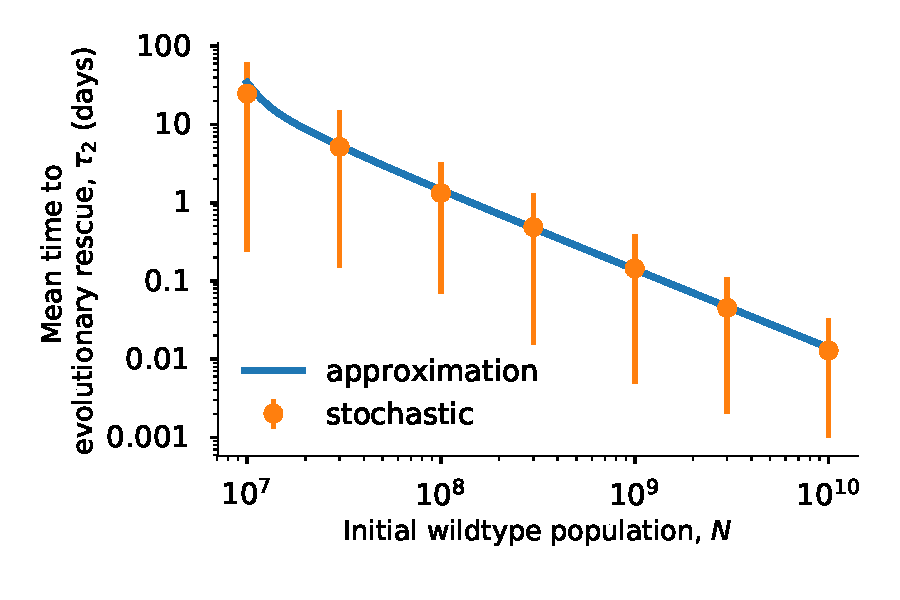
\includegraphics[width=1\textwidth]{Figures/MeanTimeDeleteriousPlot.pdf}
\end{subfigure}
\begin{subfigure}{0.5\textwidth}
B\\
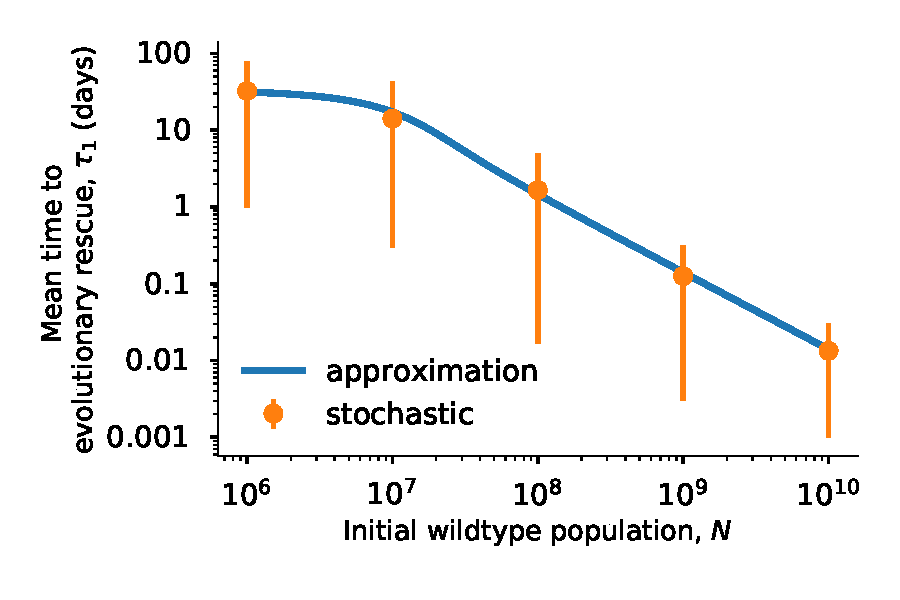
\includegraphics[width=1\textwidth]{Figures/MeanTimeGrowthMutantDirectPlot.pdf}
\end{subfigure}
\caption{\textbf{Evolutionary rescue time.}
Shown is the mean time for appearance of a resistance mutation the leads to evolutionary rescue \textbf{(left)} with aneuploidy ($u>0$) and \textbf{(right)} without aneuploidy ($u=0$).
Our inhomogeneous Poisson-process approximations (solid blue lines, right: \cref{eq:meantime1}, left: \cref{meantimet2}) is in agreement with simulation results (orange markers with 95\% CI). 
%Our 1st-order (dashed red lines, right: \cref{eq:limitapprox}, left: \cref{limitapprox2}) and 2nd-order (green line, left: \cref{limitapprox3}) approximations work well when the initial tumor size is large (here $>10^8$ cells).
Parameters: $\lambda_w=\lambda_a=\lambda_m=0.14$; $\mu_w=0.17$; (A) $\mu_a=0.145$; $\mu_m=0.13$; $u=10^{-2}$; $v=10^{-7}$.
}
\label{MeanTimeGrowthAneuploidyPlot} 
\end{figure}

\begin{figure}[!htb]
 \vspace*{1\baselineskip}
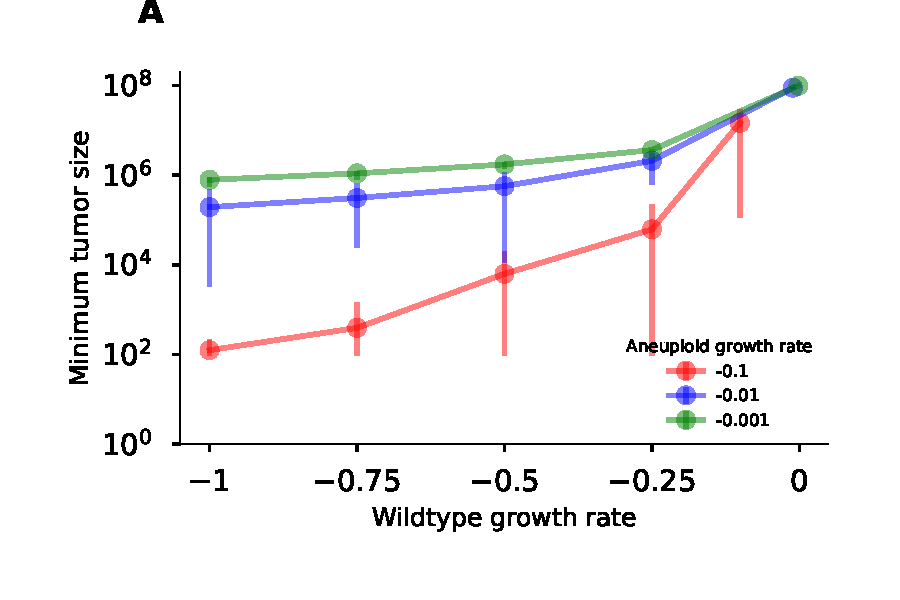
\includegraphics[width=1\textwidth]{Figures/ThresholdPopulationSize.pdf}
\caption{Minimum size that a tumor, which is exposed to chemotherapeutic drugs, reaches before adaptation sets in and tumor begins growing.
}
\label{MinTumorSize}
\end{figure}


%\begin{figure}[!htb]
%\begin{subfigure}{0.5\textwidth}
%% non-growing slightly declining, compare 1st order approximation to exact and simulation
%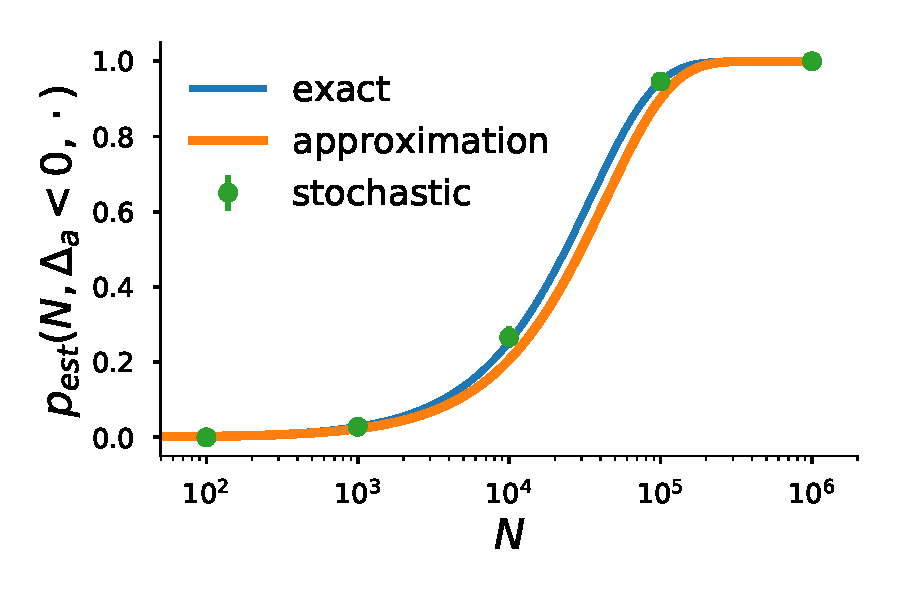
\includegraphics[width=1\textwidth]{Figures/DeleteriousTauLeapPlot.pdf}
%\end{subfigure}
%\begin{subfigure}{0.5\textwidth}
%% density-dependent simulations, barely growing (or maybe partial resistance), with exact formula
%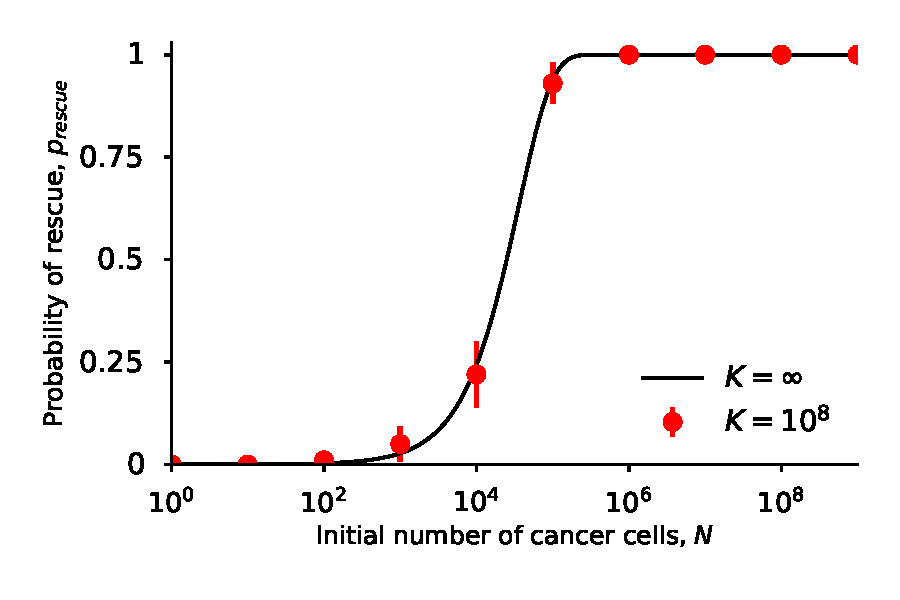
\includegraphics[width=1\textwidth]{Figures/SurvPlotNDataLogisticK.pdf}
%\end{subfigure}
%\caption{\textbf{Evolutionary rescue probability for variable initial tumor size.}
%\textbf{(A)} Comparison of simulation results (markers with 95\% CI, too small to appear with $10^5$ simulations per marker), the exact formula (blue line, \cref{eq:survival_prob} in \cref{eq:rescue_prob}) and the approximate formula (orange line, \cref{rescue_prob_approx}).
%\textbf{(B)} Comparison of results of simulations  with density-dependent growth (markers with with 95\% CI) and the exact formula (blue line, \cref{eq:survival_prob} in \cref{eq:rescue_prob}) with maximum carrying capacity $K=10^9$.
%Parameters: $\lambda_w=\lambda_a=\lambda_m=0.14$; $\mu_w=0.17$; (A) $\mu_a=0.15$, (B) $\mu_a=0.135$; $\mu_m=0.13$; $u=10^{-2}$; $v=10^{-7}$.
%}
%\label{rescue_prob_N}
%\end{figure}

\end{appendices}

%%%%%%%%%%%%%%%%%%%%%%%%%%%%%%%%%%%%%%%%%%
\end{document}